
\chapter{Generation of Meshes for the Multiscale Models}
Multiscale modeling of skeletal muscles describes phenomena on different length scales and combines them into a single description. The phenomena are modeled by different sets of equations, which need individual discretizations and solvers. Therefore, various geometrical meshes of several physical domains are required.

The considered descretization involves three-dimensional (3D) and one-dimensional (1D) meshes.
The solids of muscle and tendon are treated as 3D domain. Muscle fascicles and myofibrils are represented by 1D fibers that are embedded in the 3D domain of the muscle.

Generation of these meshes should start from biomedical imaging data in order to represent actual human anatomy. The generated meshes should be of good quality such that finding numerical solutions with low errors is made possible. It should also be possible to easily partition the mesh into multiple, equally sized subdomains. This is required for efficient parallel computation.
The latter two requirements lead to the decision to employ hexahedral elements in a structured mesh for the 3D domains.

\section{Overview and Notation of Required Meshes}
In the following, we summarize the present meshes and introduce their notation for the following discussions.

The domain of the muscle belly is denoted by $\Omega_M$. A layer of fat and skin tissue is located on top of the muscle belly. It is denoted as the body domain $\Omega_B$.
The muscle belly is attached to tendons on both longitudinal ends. The tendon domains are denoted $\Omega_{T,1}$ and $\Omega_{T,2}$. These domains are all subspaces of the 3D Euclidean space, $\Omega_M,\Omega_B,\Omega_{T,i} \subset \R^3$.

Additionally, a number $n_f$ of individual muscle fibers $\Omega_{F,i} \subset \R^3$ for $i \in \{0,\dots,n_f\}$ is introduced. Each fiber is a 1D manifold embedded in the 3D domain, i.e., $\Omega_{F,i} \subset \Omega_M$. \Cref{fig:fibers_domains} summarizes the notation of the domains.

\begin{figure}%
    \centering%
    \def\svgwidth{8cm}%
    \input{images/fiber_creation/domains.pdf_tex}%
    \caption{Visualization of the computational domains: tendons $\Omega_{T,1}, \Omega_{T,2}$, muscle belly $\Omega_M$, body domain $\Omega_B$ and fiber domains $\Omega_{F,i}$.}%
    \label{fig:fibers_domains}%
\end{figure}%

For application of the Finite Element Method, we create meshes for each of these domains. Formally, a 3D mesh $\Omega_\text{3D}$ is given by a number of 3D elements $\{U_{\text{3D},i}\}_{i=1,\dots,n}$ with $U_{\text{3D},i} \subset \R^3$ such that their disjoint union approximates the domain,
$\dot{\bigcup}_{i=1}^{n} U_\text{3D} \approx \Omega_\text{3D}$. Similar holds for 1D meshes.

The elements are non-overlapping and can be defined by nodes and edges. In the discretizations used here, no hanging nodes are allowed, i.e., at any node all adjacent elements share the node.

Furthermore, only structured, hexahedral meshes are considered in this section.
A 3D structured mesh is isomorphic to a 3D cartesian grid with equidistant elements. 
This has advantages for programmatically indexing nodes and elements as well as for parallel partitioning of the domain.

The number $n$ of 3D elements is the product of the numbers $n_i, n_j$ and $n_k$ of elements in the three coordinate directions $x,y$ and $z$ of the cartesian grid,
 i.e., $n = n_i\,n_j\, n_k$.
Each element can be indexed by a triple $(i,j,k)$ of indices with the ranges $i \in \{0,\dots,n_i-1\}, j \in \{0,\dots, n_j-1\}$ and $k \in \{0,\dots,n_k-1\}$. 
In the program, typically, consecutive indices $\iota$ are used that iterate over all elements $\iota \in \{0,\dots,n-1\}$ and are obtained from the index triples by the mapping 
$(i,j,k) \mapsto \iota = k\,n_i\,n_j + j\,n_i + i$.

The elements of such a mesh can have different numbers of nodes depending on the desired spatial order of consistency of the Finite Element discretization. The number $n_{\text{el,}d\text{D}}$ of nodes in a $d$-dimensional element is computed from the number of nodes $n_{\text{el,1D}}$ along one edge of the element as $n_{\text{el,}d\text{D}} = n_{\text{el,1D}}^d$.
Consequently, linear elements have two nodes in 1D meshes and eight nodes in 3D meshes. Quadratic elements have three nodes in 1D and 27 nodes in 3D.

It is sufficient to develop a method for constructing structured 3D meshes with linear elements. 
Higher order elements can be composed geometrically by using the nodes of multiple adjacent linear elements.
Therefore, we always generate meshes with an odd numbers $n_i,n_j$ and $n_k$ of elements in the coordinate directions first. Then, linear and quadratic meshes can be extracted from the set of nodes. Similarly, a linear 1D mesh with an odd $n_i$ can be easily converted into a quadratic 1D mesh.

The next subsections describe workflows and algorithms to construct 3D meshes for the domains $\Omega_M,\Omega_B,\Omega_{T,i}$ and 1D meshes for the fibers $\Omega_{F,i}$ following anatomical information.

\section{Related Works}

Generating volumetric meshes for domains enclosed by a given surface is a task that is frequently needed. It occurs as preprocessing step whenever spatially discretized models should be solved numerically. In consequence, numerous literature has addressed this algorithmic task and various approaches and methods have been proposed. Moreover, numerous software packages that solve this problem exist. Especially tools for computer added design and engineering as well as free or commercial preprocessing tools or Finite Element solver software include the functionality to generate meshes from given surfaces.

An example from the biomechanical domain is \cite{untaroiu2013finite}. This study develops a finite element model of the lower limb of a an occupant of a car with the aim to investigate injury scenarios during traffic crashes.
The lower extremity geometry was obtained by computer tomography (CT) and magnetic resonance imaging (MRI) scan data of a 50th percentile male volunteer. Different meshes of bones and ligaments were created using the three tools IA-FEMesh, TrueGrid and Hyper-Mesh which will be outlined in the following.

\emph{IA-FEMesh} (University of Iowa, Iowa City, USA) is an open-source tool to generate hexhedral meshes \cite{grosland2009ia}. The user is presented with an interactive environment where existing geometries can be loaded. In a visualization, bounding cuboids, called blocks, can be positioned around the geometry. A structured grid on the block is then projected onto the surface of the geometry. Multiple blocks can be placed to account for more complex geometry. The surface mesh is improved using Laplacian smoothing which equalizes the edge lengths of the elements.
The interior nodes are generated using interpolation.
The result will be a structured mesh if only one block is used or an unstructured mesh if multiple blocks are used. Further operations to manage mesh density, visually manipulate the meshes and add material properties, loading and boundary conditions are available. The model can be exported in a file format for Finite Element analysis with ABAQUS.

The second tool is \emph{TrueGrid} (XYZScientific Applications, Livermore, USA). It is a commercial toolkit to generate hexahedral meshes. The project was started in the early 1990s as the successor to the even older preprocessor software \emph{INGRID}. The user interface still feels like being from those older times. Similar to \emph{IA-FEMesh}, a projection method and multi-block technique is used. Some effort has been put into dealing with holes and sewing together dissimilar blocks.

The third tool is \emph{Hyper-Mesh}, the commercial pre- and postprocessing toolkit of Hyperworks (Altair HyperWorks, Troy, USA).
Altair sells infrastructure and solvers for a multitude of physics and is targeted at a wide range of industries. 
Therefore, information about the internals of their preprocessing software are hardly available.

More meshing software exists, such as CGALmesh \cite{Jamin2015CGALmesh} for tetrahedral meshes. The package gives quality guarantees of their generated meshes and include four mesh optimization algorithms to further improve the mesh quality.

Another work dedicated to the use of commercial tools is \cite{Ellankavi2018}. A workflow for patient-specific modelling, simulation and analysis of the interaction between a residual lower limb stump and the socket of a prosthesis is presented. Imaging data was taken from magnetic resonance diffusion tensor imaging where also the preferred diffusion direction of water molecules along muscle fibers is captured. The open-source tool MedInria (National Institute for Research in Digital Science and Technology (Inria), France) \cite{vichot2012cardiac} was used to extract muscle fibers. The residual limb data was processed using the commercial 3D image segmentation software Simpleware ScanIP (Synopsys, Mountain View, USA). Auxiliary tasks were performed using MATLAB (MathWorks,	Natick, USA) scripts. The commercial multiphysics solver LS-DYNA (LSTC/Ansys, Canonsburg, USA) was used for the simulations.

Commercial tools usually have the advantage that more development effort was put into them, than is possible for open-source codes from the scientific community. This often leads to more robust and user-friendly software. An advantage of open-source software is that the used algorithms are transparently visible. They are often well documented or described in a publication. This allows to assess the expected quality of the generated meshes. Conversely, commercial vendors usually have no interest in revealing their internal algorithms.

For our simulation, structured hexahedral meshes are needed. Several of the described tools are able to generate hexahedral meshes, however the meshes are often unstructured. For our special need of 1D muscle fibers embedded in a 3D mesh, we develop our own method that is based on the ideas of existing algorithms.

% other 3D meshing
% tets
Triangulating a 2D domain is the archetype of mesh creation. The triangulation named after B. Delaunay was formulated in 1934 \cite{delaunay1934sphere}. For a given set of points, it maximizes the minimum angle of the triangles and, thus, avoids small angles. Therefore, a guarantee on the quality of the triangulation is given.

In 1995, J. Ruppert presented the Delaunay refinement algorithm \cite{Ruppert1995}, which constructs a Delaunay triangulation conforming to prescribed connected points. This algorithm is still commonly used and also part of derived meshing techniques.

In 1997, P. Chew developed an algorithm for meshing a 3D domain with tetrahedra \cite{chew1997guaranteed} and proved that thet aspect ratio of the tetrahedra is bounded, i.e., degenerate, \say{flat} tetrahedra, called slivers are avoided.

The authors of \cite{Alliez2005Variational} propose a variational approach to meshing where a quadratic energy function is minimized. During minimization both vertex positions and connectivity are optimized. This leads to better quality meshes than by simple Delaunay triangulation.

% tets to quads:
Hexahedral meshes can be obtained from certain tetrahedral meshes by splitting up each tetrahedron into four hexahedra. This is discussed in \cite{eppstein1999linear}. A remaining issue is that the generated meshes from this procedure are highly unstructured and some hexahedra have poor quality. Instead, the goal is to construct elements that are almost equilateral.

A different approach is to directly generate a hexahedral mesh for the given surface geometry.
The survey in \cite{owen1998survey} identifies four different strategies for generating unstructured hexahedral meshes.

The first one is a \emph{grid-based} approach. It was introduced in \cite{schneiders1996grid,schneiders1997algorithm}. The interior of a given solid is filled with a grid of as many hexahedral elements as fit into the space. Then the gaps at the surface are filled with additional elements. This method is robust but can lead to poor quality elements near the surface. The orientation of the interior grid highly depends on the orientation of the initial surfaces and may not be the natural orientation of the given volume.

The second approach for generation of hexahedral meshes are \emph{medial surface methods} \cite{price1995hexahedral, price1997hexahedral}. First, the volume is decomposed into subregions by medial surfaces such that the resulting domains are one of only 13 possible types. Predefined templates are used to fill the domains with hexahedral elements. Then, the continuity between the domains is ensured using linear programming. This approach gives good results for some geometry but has robustness issues for general geometry.

The third approach is called \emph{plastering}. It was first described by \cite{blacker1993seams} and continued by \cite{staten2006unconstrained,staten2010unconstrained}.
It is a moving-front method where hexahedral elements are placed in layers starting at the border and moving towards the interior. Intersection of faces has to be detected when the fronts meet in the interior and rules for connecting to existing faces have to be defined.
During this process, complex shaped voids can occur in the interior. When it is no longer possible to fill the voids with hexahedrons already placed elements have to be removed.
A new method, called unconstrained plastering, starts from an unmeshed volume boundary. The approach has general robustness issues and is not guaranteed to find a solution for arbitrary boundary.

The forth approach is \emph{whisker weaving}, introduced by \cite{tautges1996whisker} and extended by \cite{ledoux2008extension,kawamura2008strategy}. The dual of the hexahedral mesh is considered. The dual consists of the three surfaces per hexahedron that lie in the planes of symmetry. The surfaces of all hexahedrons form topological loops. 
The principle is now to first construct the dual of the mesh, which can be easily determined from the given boundary surface. Then, the actual hexahedral mesh can be created from the dual, using the surfaces as guides where to place the elements.
The dual forms topological loops inside the volume. One important criterion for generating good quality meshes is that self-intersections of these loops are resolved in a first step.
The approach, used with subsequent smoothing, can produce meshes of good quality. However, no guarantee is given. One problem is that the resulting mesh depends on the quality of the surface mesh and that the number of nodes can increase significantly during the method.

For the whisker weaving method and for some plastering methods, a quadrilateral mesh of the surface is required. Algorithms for creating high quality quadrangulations of closed surfaces exist \cite{dong2005quadrangulating,Kovacs2011Anisotropic,Bessmeltsev2012,Meng2016Consistent}.

Other approaches start with 3D volumetric medical imaging data instead of surfaces. In \cite{Zhang2003,Zhang20053DFiniteElementMeshing}, adaptive tetrahedral and hexahedral meshes are created from volumetric data using octree subdivision. The method avoids hanging nodes and allows a feature sensitive adaptivity. While adaptive meshing methods can reduce the number of elements in the interior of the volume, a problem is that the worst quality elements are generated at the border, the location where the solution in a Finite Element study usually is the most interesting.

Multiple reasons make the previously outlined approaches unsuited regarding the needs for our parallel muscle simulation. 

(i) The generated meshes are unstructured. When performing domain decomposition for parallel computing, graph-partitioning methods have to be used. Storing an unstructured mesh requires storage of element adjacency information. Partitioned meshes additionally require storage of the adjacent processes. Structured meshes can be trivially decomposed and stored efficiently. A decomposition can be represented in memory by a very low number of constant properties.

(ii) The presented methods are designed for hexahedral meshing of arbitrary volumes. Robustness and mesh quality at the same time remain issues that are not completely solved for most of the algorithms. Often, expensive smoothing steps are needed to increase mesh quality.

(iii) In general, either no assumption can be made about orientation or alignment of hexahedrons in the interior, or, for the grid-based approach, the elements at the surface have poor quality. Having a mesh that is consistently aligned with, e.g., the main diffusion direction or the preferential direction of the anisotropic material can reduce numerical errors in the Finite Element solution.

Consequently, a more scenario specific solution is needed. An example is \cite{blemker2005three}, where 3D Finite Element models for various complex muscle geometries  around the hip are generated from magnetic resonance images. Segmentation and surface mesh generation are performed using the old, unmaintained software \emph{Nuages} (Inria, France).
A 3D hexahendral mesh is generated using TrueGrid. A structured template mesh on a unit square is mapped to the horizontal slices of the muscle geometry that resulted from the segmentation. After mesh smoothing, the slices are connected vertically to form a 3D mesh. 

Fiber directions are described by Bezier curves in a reference volume and mapped to the muscle geometry using the same mapping. The fiber direction then are used in a transversely-isotropic material formulation. Simulations are performed using the Finite Element solver \emph{Nike3D} (Lawrence Livermore National Lab, Livermore, USA) \cite{Nike3D}.

We base our work on this study and use a similar mapping from a template mesh to the actual muscle volume. Contrary to \cite{blemker2005three}, we improve this mapping by using harmonic maps, which potentially leads to better quality meshes on the slices of the muscle. Instead of the unit circle template mesh, we experiment with different reference meshes and evaluate their quality.

In the study of \cite{blemker2005three}, fiber directions are defined based on anatomically assumed directions.
However, the definition is carried out on the cuboid reference geometry. This means that the authors mentally morph the muscle geometry into the reference geometry in order to define fiber directions, using their expertise. Then, the fiber directions together with the cuboid are transformed back to the actual geometry. This approach simplifies the definition of the fibers. However, defining the fiber direction directly on the muscle geometry can lead to better results. 

Our approach is to estimate fiber directions and define fibers directly in the muscle domain. At the same time, the 3D mesh and 1D fibers are aligned to allow for better numerical properties of the discretization. 

The definition of fiber directions follows a method proposed in \cite{Choi2013}. 
The directions are assumed to follow a divergence free vector field. Such a field can be created by taking the gradient of the solution of the Laplace equation. Neumann boundary conditions are defined at the attachment points of the muscle tendon complex. The solution of the Laplace equation corresponds to the pressure values of a potential flow. Its gradient corresponds to the velocity and individual fascicles or fibers can be obtain by tracing streamlines through the velocity field.
This approach is extendend and validated by the studies in \cite{Inouye2015} and \cite{Handsfield2017}. We incorporate this method into our workflow.

\section{Preprocessing of the Muscle Geometry}

The first step towards creating a structured mesh is to obtain a representation of the surface of the muscle. 
Starting point is a human biomedical imaging data set. In this section, two possible workflows are presented how to extract the muscle and tendon surface. 
The two workflows are visualized in \cref{fig:scheme_preprocessing}. The workflow using the branch on the left side in \cref{fig:scheme_preprocessing} is automized but only works for the particular data set and extracting the biceps muscle.
The right branch involves manual steps and is applicable for any muscle geometry.

% overview over subsections

\begin{figure}%
  \centering%
  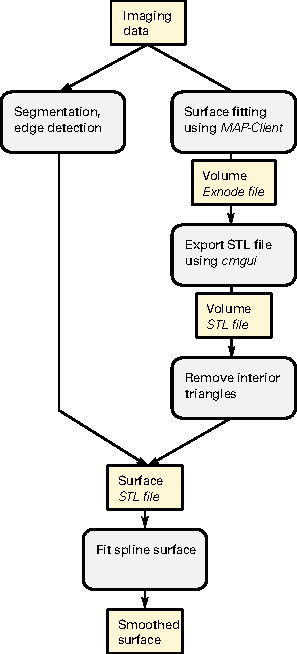
\includegraphics[height=15cm]{images/fiber_creation/scheme_preprocessing.pdf}%
  \caption{Workflow of generating a surface representation of the muscle and tendons from imaging data. Intermediate results are visualized as yellow boxes. Two possible branches are shown. On the left, the imaging data is processed using automatic processing to directly retrieve points on the surface of the muscle. On the right, the same is achieved with three steps of which the first one involves manual adjustments. At the end, a spline surface smooths the collected data from both possibilities to yield the resulting surface representation.}%
  \label{fig:scheme_preprocessing}%
\end{figure}%

\subsection{Data source}
Anatomic images provide the basis for the extraction of muscle geometries.
The used data set originates from the Visible Human Project \cite{visible_human_male} of 
the United States National Library of Medicine. 
The project has published anatomic images derived from a male cadaver, among other data sets.
The data, known as \say{Visible Human Male}, were published in 1994.
Colored images of transversal cross sections were obtain by cryosectioning.
A total of \num{1871} images with dimensions of \num{2048} by \num{1216} pixels and 24 bit color depth visualize the whole human body. Parts of the upper arms are contained in approximately 500 of these images. The size of a pixel is \SI{0.33}{\milli\meter} in transversal direction and \SI{1}{\milli\meter} in axial direction. The size of the complete set of JPEG compressed images is \SI{772}{\mega\byte}. Cropping and selecting the relevant portions of the upper arm extracts a dataset with the size of \SI{35}{\mega\byte}.

An extract of an image of the upper arm is given in \cref{fig:vhp_image}. 
Biceps and triceps brachii muscles can be identified as the dark red tissue. For the biceps, the two muscle heads are visible, separated by the bright diagonal line from bottom left to top right. For the triceps, at least two of the three heads can be identified. The blue background is colored frozen gelatin that was needed during cryosection to stabilize the arms.

\begin{figure}%
  \centering%
  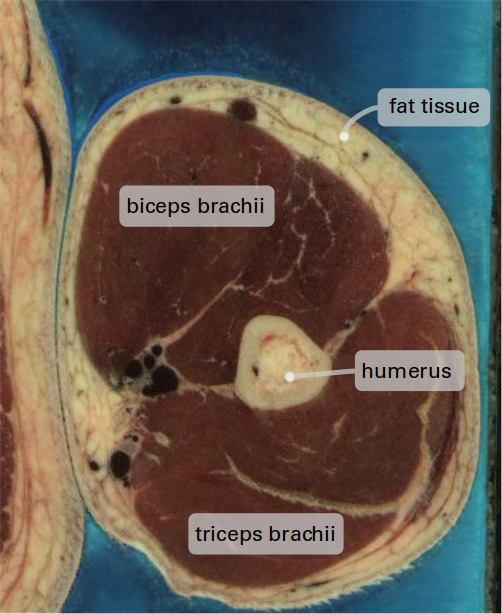
\includegraphics[height=10cm]{images/fiber_creation/vhp.png}% 0483
  \caption{Exemplary extract of image number 483 from the Visible Human Male. A transversal slice of the left upper arm is shown as seen from the bottom. The biceps and triceps muscles as well as the humerus bone can be identified. }%
  \label{fig:vhp_image}%
\end{figure}%

\subsection{Automatic surface extraction}
This section outlines the automatic algorithm to obtain the muscle surface from the Visible Human Male data set. The scheme corresponds to the left branch in \cref{fig:scheme_preprocessing}. The algorithm was implemented as Python script as part of the Bachelor thesis of Kusterer \cite{Kusterer} that was supervised by me.
The algorithm is capable of extracting muscle and bone geometries from the described imaging data.

At first, the color values of the images are used to segment the imaging data into muscle tissue, surrounding tissue and skeletal structure. The algorithm traverses the selected and cropped relevant parts of the images. For example, to segment the biceps muscle, the image region of pixels coordinates $(x,y)$ with $x \in [1300,1720] $ and $ y\in[1030,1720]$ are considered in the images with numbers 284 to 778. 

For every such part of an image, pixels that match a certain range in the RGB color space are marked and categorized. The categories are muscle tissue and, for comparison, also bone tissue. The corresponding color ranges are given in \cref{tab:color_ranges}.
This color based classification does not succeed everywhere as the white shade corresponds not only to bone material but also to fat and other tissue. Therefore, the algorithm removes artifacts located near the outer gelatine from the set of pixels categorized as bone. 

\begin{table}
  \centering%
  \begin{tabular}{l|lll}
    \hline
    & red & green & blue\\
    \hline
    muscle & $60 - 100$& $30-75$   & $15-60$\\
    bone   & $145-255$ & 1$35-205$ & $60-160$\\
    \hline
  \end{tabular}
  \caption{Ranges in the RGB color space to identify pixels of muscle and bone segments. The numbers correspond to 24 bit colors with the range $[0,255]$ for every color channel.}%
  \label{tab:color_ranges}%
\end{table}

Exemplary results for image number 483 are given in the left column of \cref{fig:vhp_image}.
It can be seen that the marked regions for muscle and bone have gaps in the interior resulting from differently colored tissue inside muscles and bones. On some images, the set of pixels also includes small objects outside the actual muscle and bone regions.

To reduce the gaps and small objects, the morphological operations \emph{closing} and \emph{opening} are performed on the data. These operations consist of \emph{dilation} and \emph{erosion} steps. Both are pixel based operations that traverse the dataset and for every pixel consider a window of $3\times 3$ pixels centered at the current position. Dilation picks the maximum value and erosion the minimum value from this window and assigns it as the pixel's value in a new image. In our case, values of zero and one correspond to non-categorized and categorized pixels, respectively.

Closing consists of dilation followed by erosion and closes small gaps or holes in the marked objects. Opening consists of erosion followed by dilation and removes small artifacts outside the actual bone and muscle areas. It was found effective to perform each dilation and erosion twice in sequence to yield good results with almost no more holes and unwanted small objects.

Next, the algorithm determines the contours of all regions with marked pixels. This leads to lines with a width of one pixel that enclose the muscle and bone areas. The right column of \cref{fig:extraction} shows the results after this step. It can be seen that the morphological operations close numerous gaps. In some images, as in the considered example, the muscle area gets split into multiple smaller enclosed regions which is not desired. However, proper contours of the biceps are found in the majority of images. 

\fboxsep=0mm   % padding thickness
\fboxrule=1pt   % border thickness
\begin{figure}%
  \centering%
  \fcolorbox{black}{black}{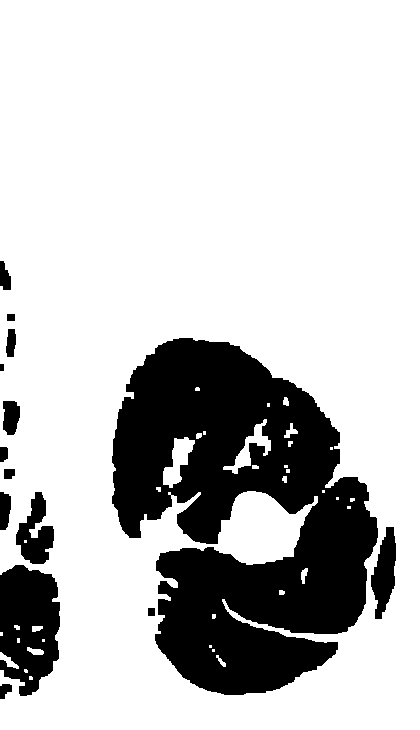
\includegraphics[height=7cm,trim=0 0 0 6cm, clip]{images/fiber_creation/extraction_segmentation_482.png}}\quad%
  \fcolorbox{black}{black}{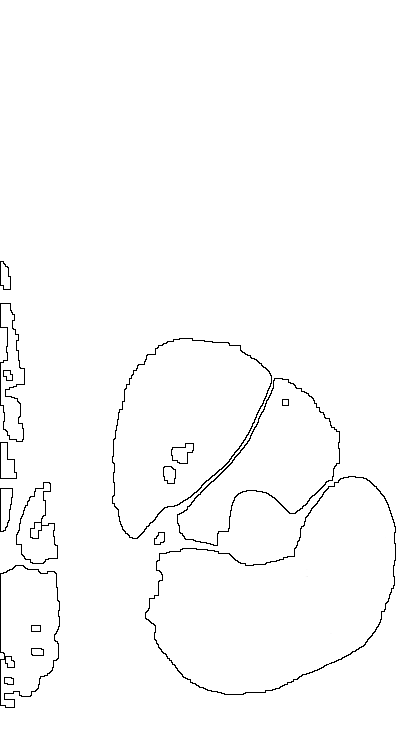
\includegraphics[height=7cm,trim=0 0 0 4cm, clip]{images/fiber_creation/extraction_contour_482.png}}\vspace*{5mm}\\
  \fcolorbox{black}{black}{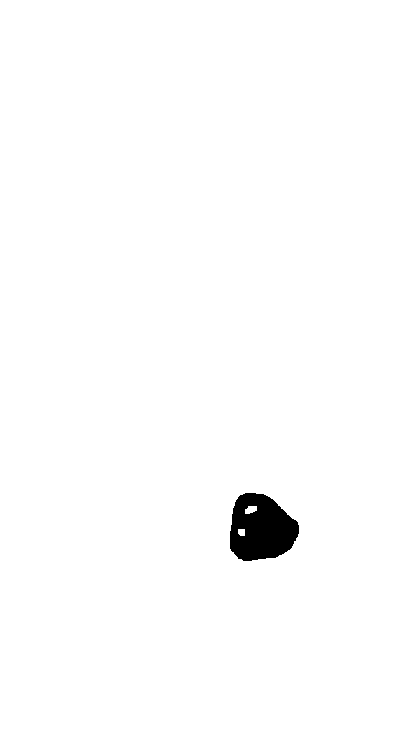
\includegraphics[height=7cm,trim=0 0 0 6cm, clip]{images/fiber_creation/extraction_bone482.png}}\quad%
  \fcolorbox{black}{black}{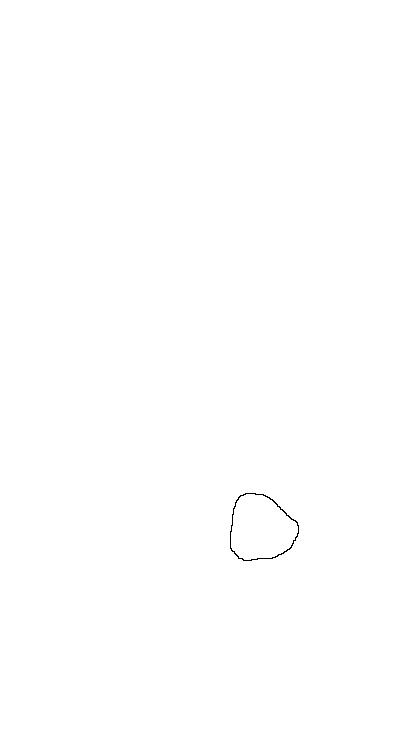
\includegraphics[height=7cm,trim=0 0 0 6cm, clip]{images/fiber_creation/extraction_surface_bone482.png}}%
  \caption{Intermediate steps of the algorithm to determine surface geometry of muscles and bones. The left columns shows pixels from the image in \cref{fig:vhp_image} that were categorized to be muscle tissue (top) and bone material (bottom). The right column shows a later step in the algorithm, where the surface of muscle (top) and bone (bottom) is estimated.}%
  \label{fig:extraction}%
\end{figure}%

In the next step, a single contour for each of muscle and bone is obtained in every image. If there are multiple contours per image, the one that is located the most in upper right location within the image is selected for the muscle. If all contours in an image are shorter than 20 pixels, this is a sign of bad segmentation quality and the whole image gets discarded.

The result is a set of contours for muscle and bone in the cross-sectional planes of the images. Combining these, we get a point cloud in 3D space that approximates the surface of the biceps muscle and the surfaces of the considered bones humerus, ulna and radius. Using these points, a spline surface can be fitted and subsequently triangulated. Resulting surfaces for the biceps and humerus bones are shown in \cref{fig:extraction_result}.
%
\begin{figure}%
  \centering%
  \begin{subfigure}[t]{0.48\textwidth}%
    \centering%
    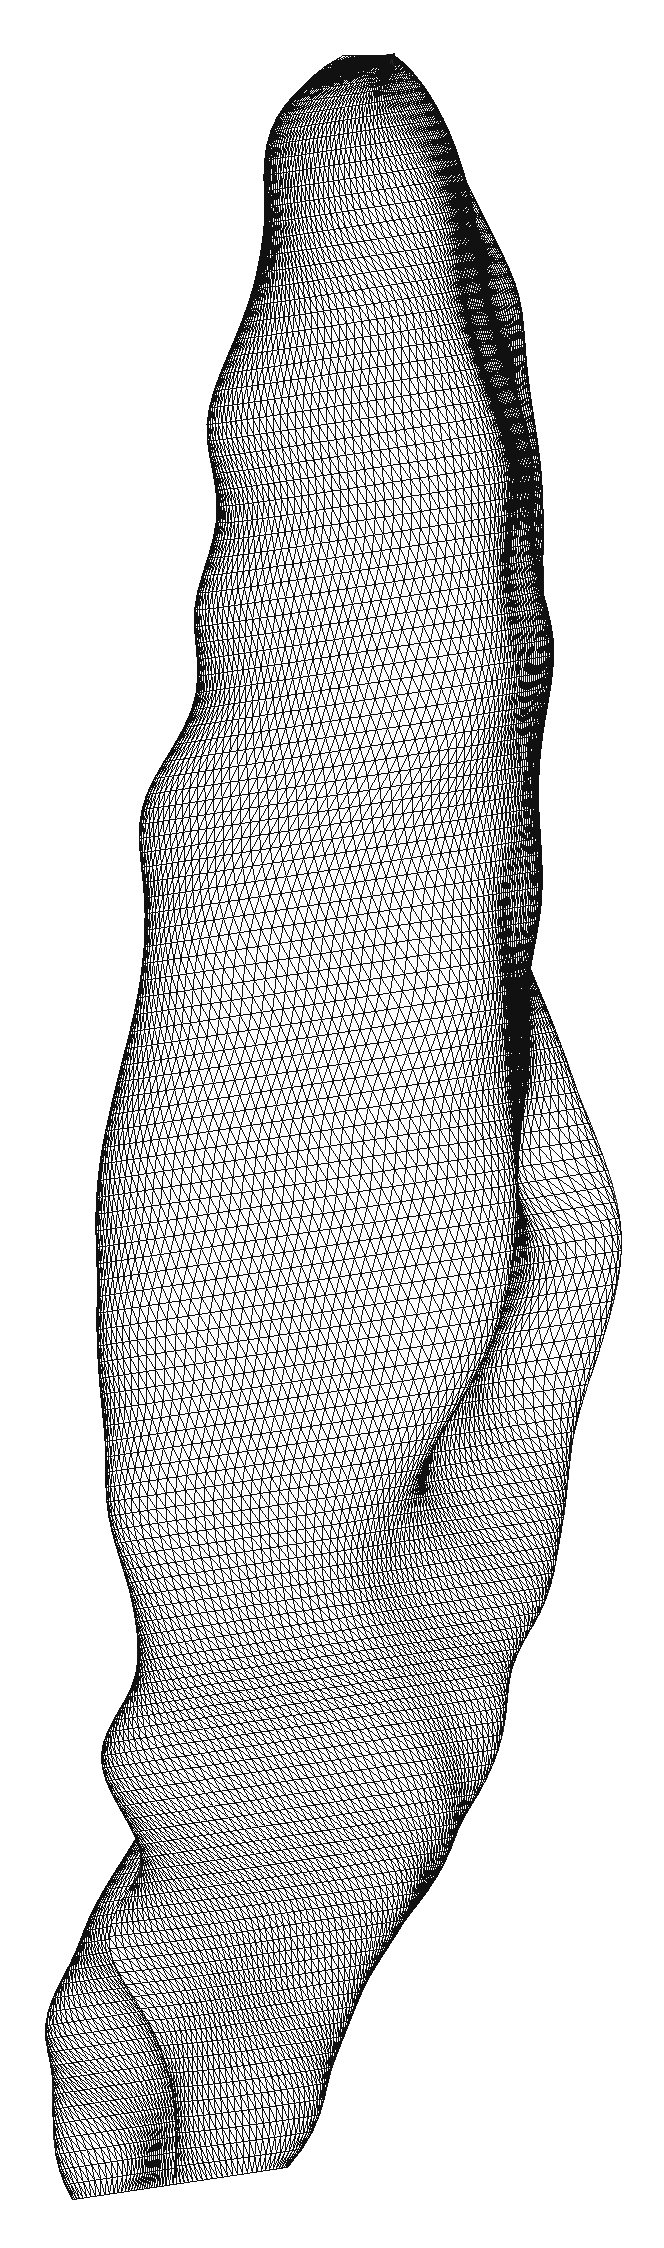
\includegraphics[height=6cm]{images/fiber_creation/extraction_biceps.png}%
    \caption{Surface of the biceps brachii muscle. At the right side of the muscle, the groove of the humerus bone can be seen.}%
    \label{fig:extraction_result_biceps}%
  \end{subfigure}
  \begin{subfigure}[t]{0.48\textwidth}%
    \centering%
    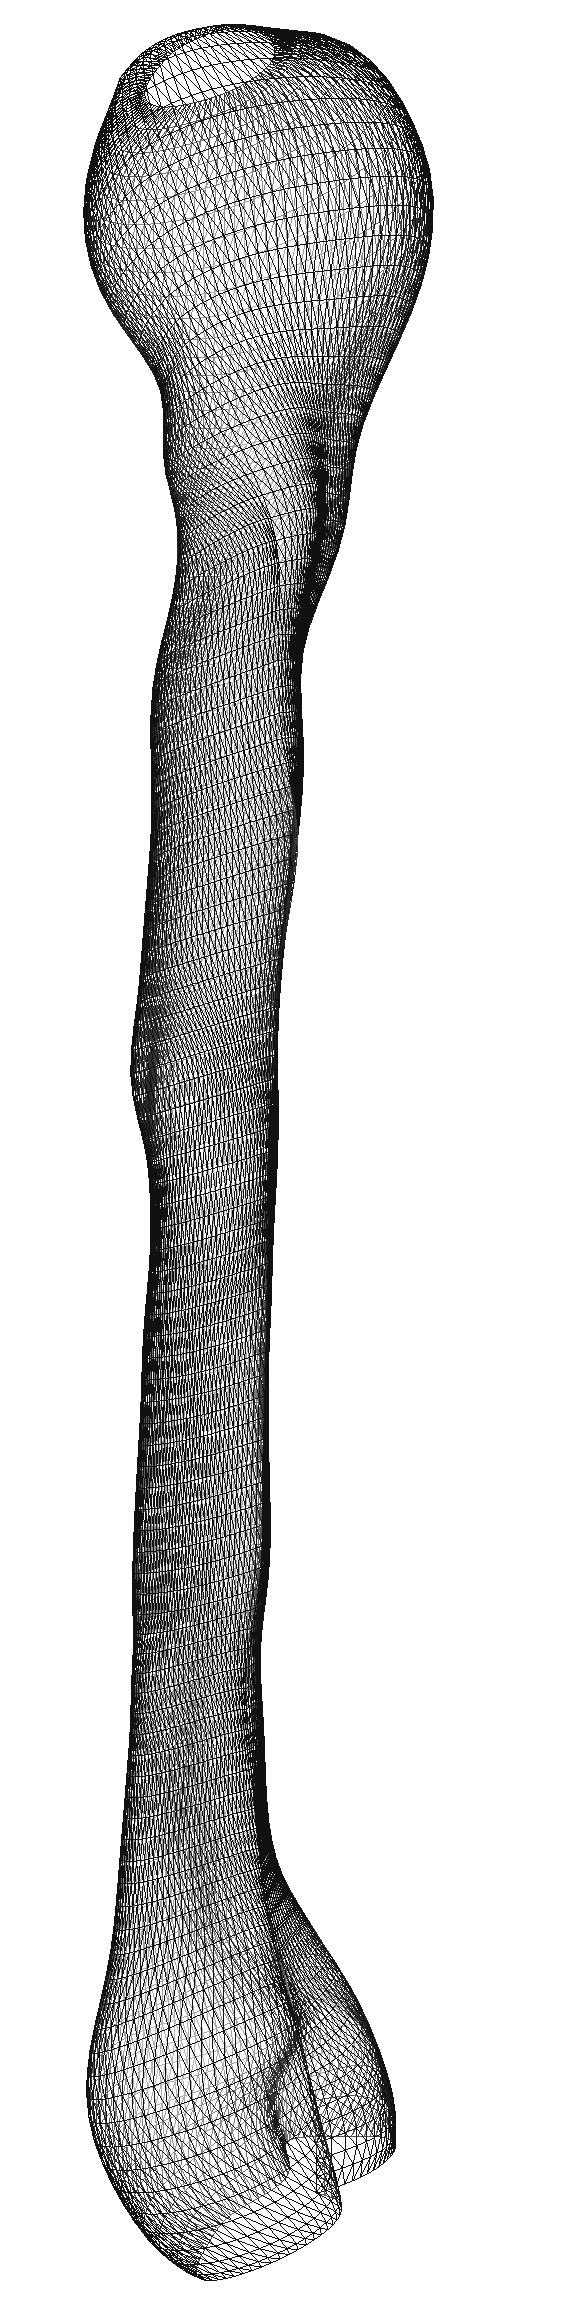
\includegraphics[height=6cm]{images/fiber_creation/extraction_humerus00.png}%
    \caption{Surface of the humerus}%
    \label{fig:extraction_result_humerus}%
  \end{subfigure}    
  \caption{Resulting surfaces of biceps and humerus bone obtained by the automatic surface extraction algorithm.}%
  \label{fig:extraction_result}%
\end{figure}%

The runtime for the algorithm is \SI{121}{\minute} on a AMD Ryzen 5 1600 processor with 6 cores, 3.2 GHz and \SI{16}{\giga\byte} RAM, of which a maximum of \SI{2}{\giga\byte} was used at maximum. Because processing of the images can be done in parallel, the runtime can be reduced to approximately half (\SI{62}{\minute}) using 2 threads and to a quarter (\SI{30}{\minute}) using 6 threads.

The advantage of the presented algorithm is that the outcome solely depends on the imaging data and, thus, no modeling error by manual approximation of the geometry occurs. For example, the obtained surfaces of biceps and humerus geometrically fit perfectly into each other. Intermediate steps are stored as black and white images. By editing these between the steps of the algorithm, manual tweaking is possible and could lead to increased quality of the results.

A disadvantage is that it relies on color information in the imaging data to differentiate between muscle and other tissue. Because the involved tissue has similar colors, these differences are often small. Furthermore, the color ranges need to be determined experimentally. Therefore, the algorithm is not very robust with respect to image noise and needs adjustments when it should be used to extract other muscles. Expert knowledge about the location and shape of human muscles cannot be used easily to improve the results of the algorithm.

A different approach is to manually segment the imaging data and construct surfaces with the help of a tool. This approach is described in the following section.

\subsection{Manually guided surface extraction}\label{sec:surf_extr}

The manually guided segmentation is done using the \emph{MAP client} of the Musculoskeletal Altas Project (MAP) \cite{mapclient}. This application allows to create and execute a workflow to achieve data processing and simulation tasks. In a graphical window, the user can place and connect various workflow steps. When executing the workflow, each step shows a dialog where the required configuration can be entered or the operations can be performed on a visual presentation of the data at this workflow stage. 

Possible workflow steps include source and sink operations such as reading image data and writing meshes. Imaging data such as the 2D images from the Visual Human Male can be visualized in a 3D representation. The user can place points in the 3D space and try to match borders of the muscles and structures to extract from the data.
Further workflow steps allow to create meshes of predefined geometrical shapes, such as cubes and cylinders and merge them into a common mesh. These meshes can be fitted to point clouds of user defined points. This is done by a least squares approach minizing the distances between user created points and the mesh surface.

The MAP client has a plugin architecture and allows to create new workflow steps. It includes features from OpenCMISS, especially data processing formats and tools from OpenCMISS Zinc. Meshes can be created with 3D cubic Hermite elements that allow a high geometric modelling flexibility with a low number of nodes. Such meshes are stored in the OpenCMISS file format of \code{exnode} and \code{exelem} files.

As a result, meshes of individual muscles or the whole human organism can be created. \Cref{fig:vhp_geometry} shows meshes that were create from the cryosectioning data of the Visible Human Male. In \cref{fig:vhp_total} almost the whole body has been extracted. In \cref{fig:vhp_detail}, the mesh consisting of cubic Hermite elements is visualized. A relatively coarse mesh width suffices to model a smooth surface of the body. When exported in the exfiles format from the MAP client, the data can be visualized, e.g., using \emph{cmgui}, the visualization tool of OpenCMISS Zinc.

\begin{figure}%
  \centering%  
  \begin{subfigure}[t]{0.48\textwidth}%
    \centering%
    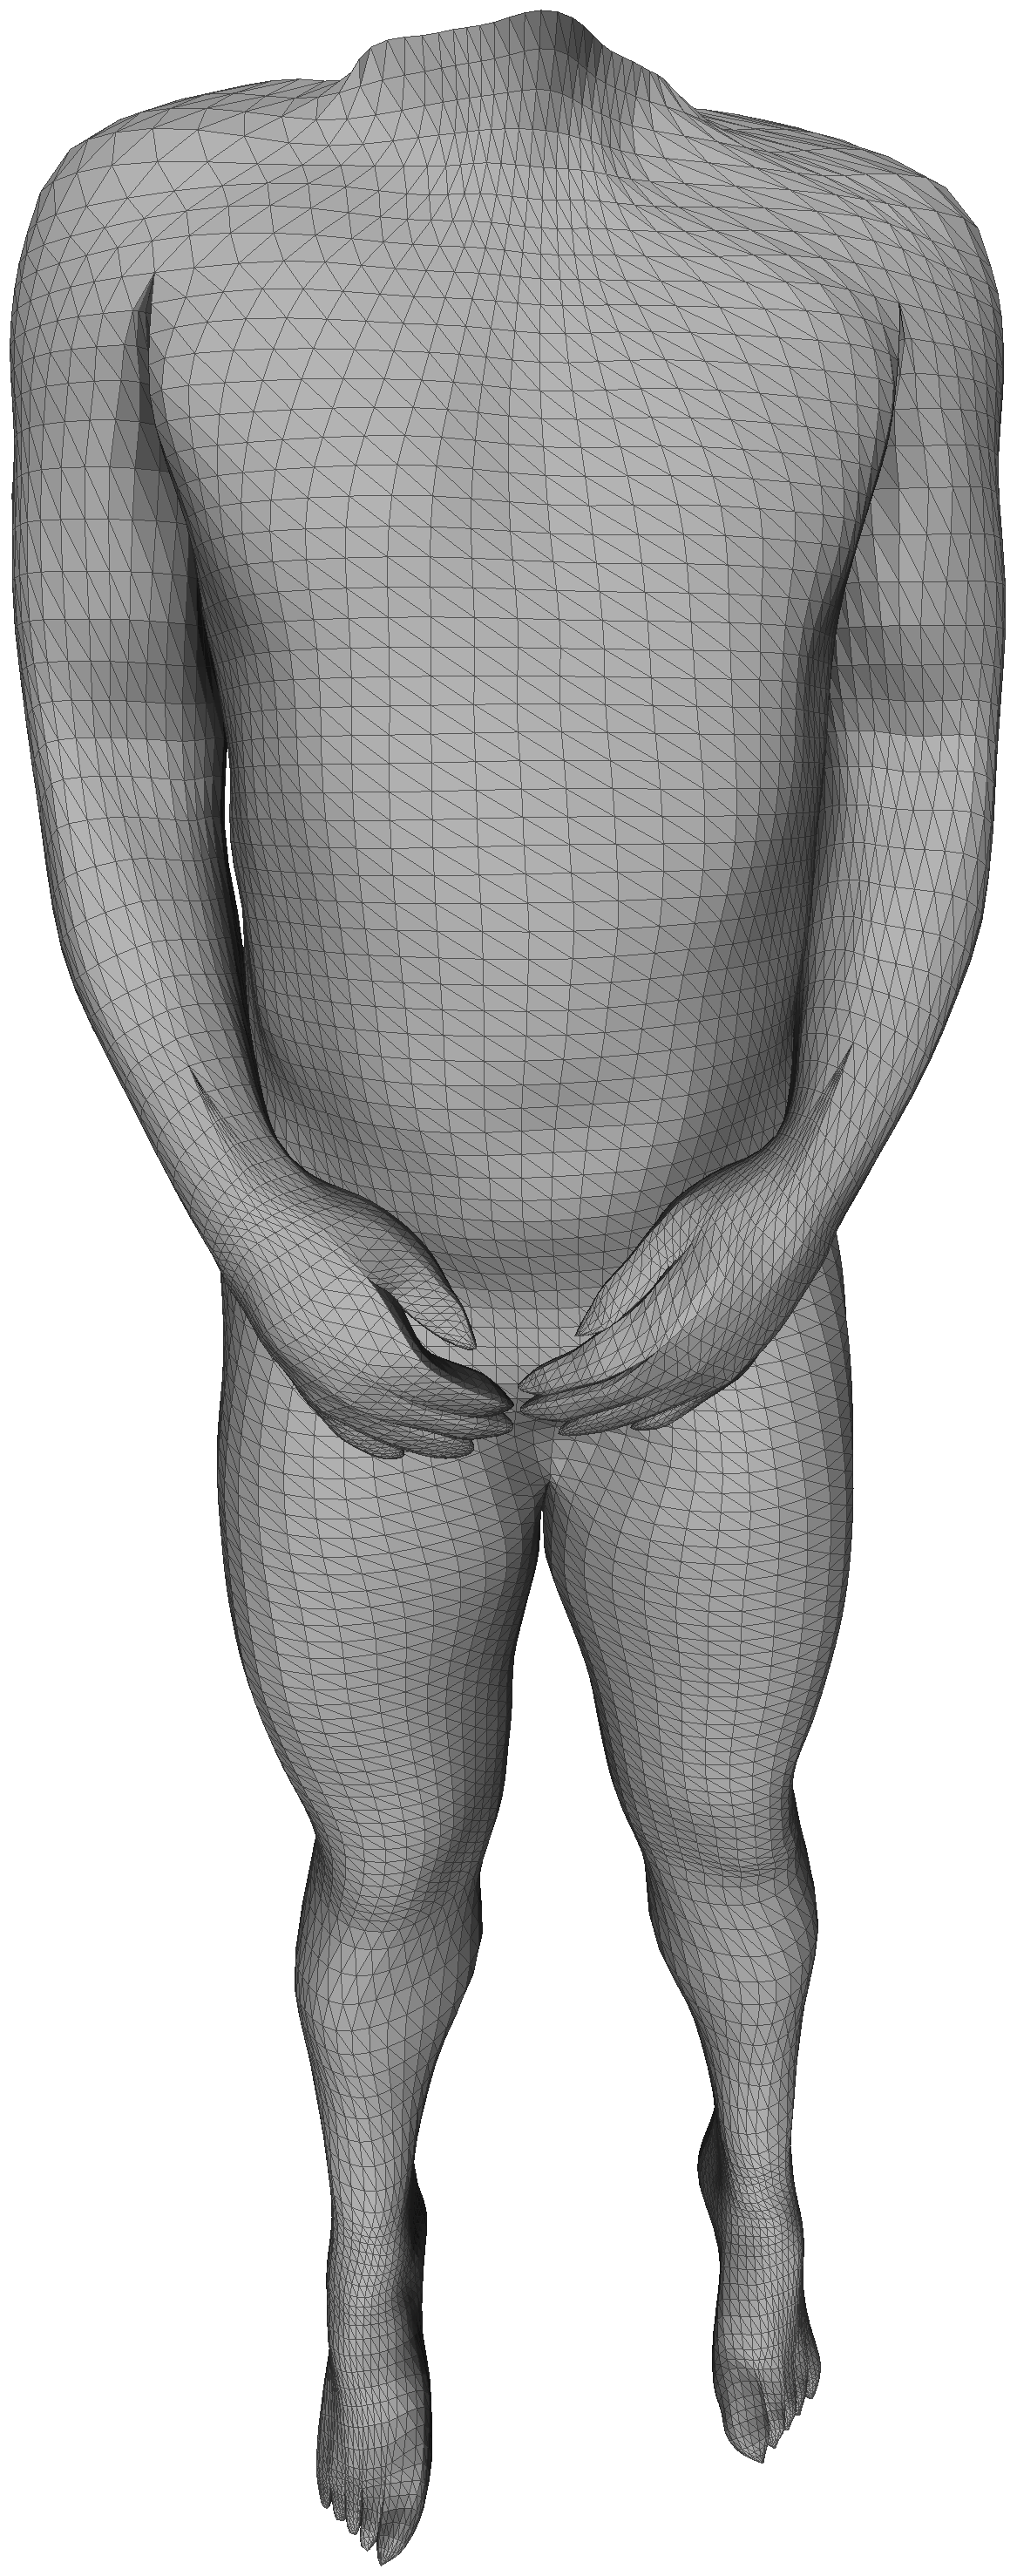
\includegraphics[height=10cm]{images/fiber_creation/skin00.png}%
    \caption{Mesh of the trunk and limbs, surface has been triangulated for visualization.}%
    \label{fig:vhp_total}%
  \end{subfigure}
  \quad
  \begin{subfigure}[t]{0.48\textwidth}%
    \centering%
    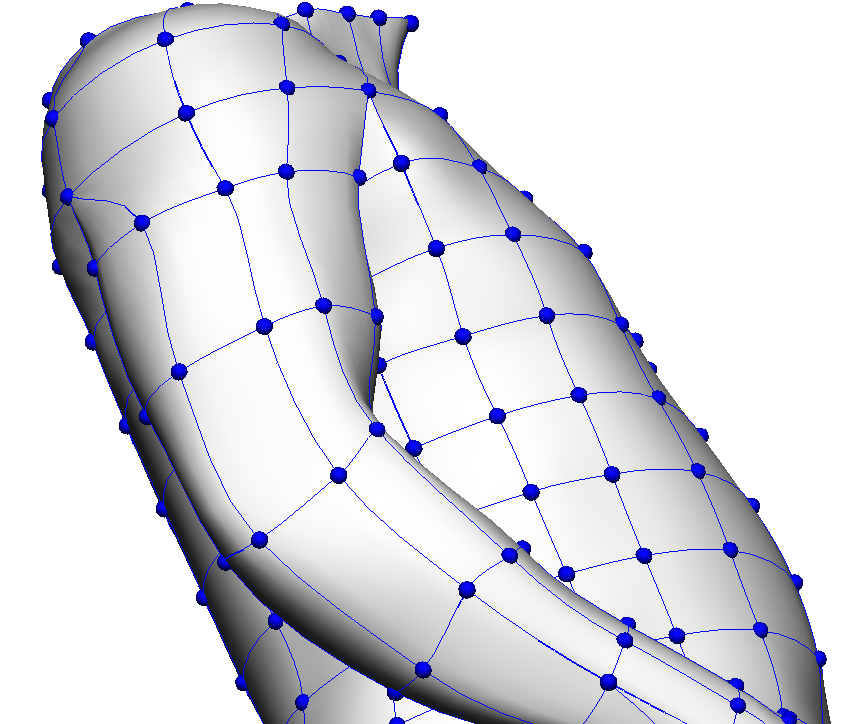
\includegraphics[height=7cm]{images/fiber_creation/elements4.png}%
    \caption{Detail view of part of the right upper arm and the trunk with blue nodes and contours of a mesh with cubic Hermite elements.}%
    \label{fig:vhp_detail}%
  \end{subfigure} 
  \caption{Mesh of the Visible Human Male from the Visible Human Project.}%
  \label{fig:vhp_geometry}% 
\end{figure}%

The mesh width of the meshes obtained using the MAP client was chosen such that the surface fitting yielded good results. The meshes are not necessarily ready for use in a simulation, especially if a  high mesh resolution is desired. 
Apart from the mesh width also the type of elements can be different than what is needed for a Finite Element simulation. Our goal is to obtain meshes with linear or quadratic Lagrange elements with configurable mesh widths for the specified upper arm muscles, such as the biceps brachii.

Therefore, the next step of the workflow, as visualized by the right branch of \cref{fig:scheme_preprocessing}, is to transform the volume mesh into a surface mesh which then can be used as basis for further meshing. This is visualized with the example of the biceps muscle in \cref{fig:biceps_processing}. The basis is the Hermite mesh shown in the left-most image.

\begin{figure}%
  \centering%
  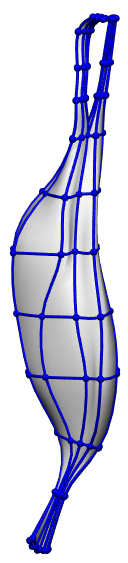
\includegraphics[height=10cm]{images/fiber_creation/exfile.png}\quad%
  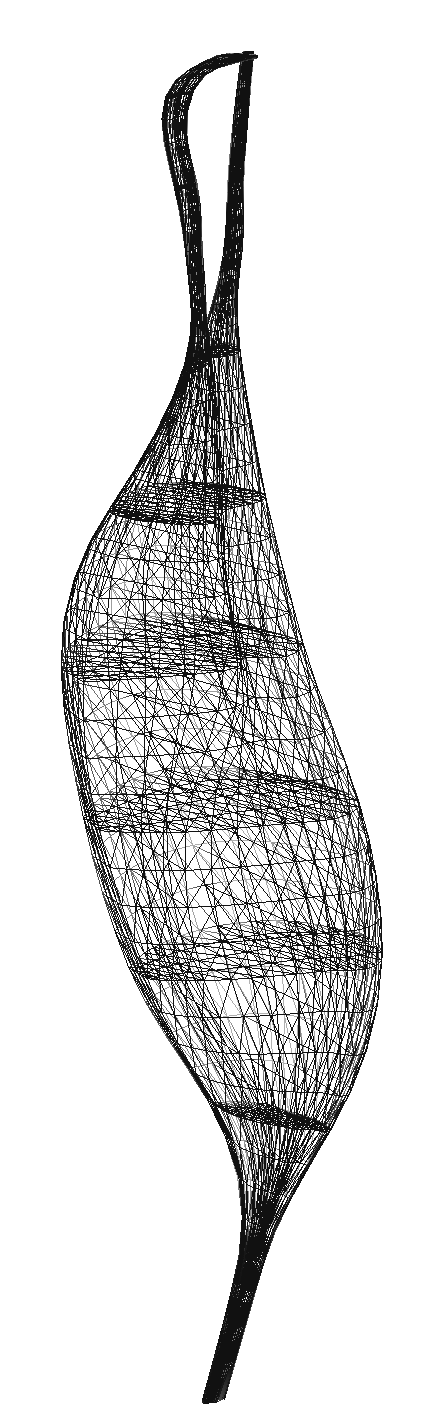
\includegraphics[height=10cm]{images/fiber_creation/biceps23.png}%
  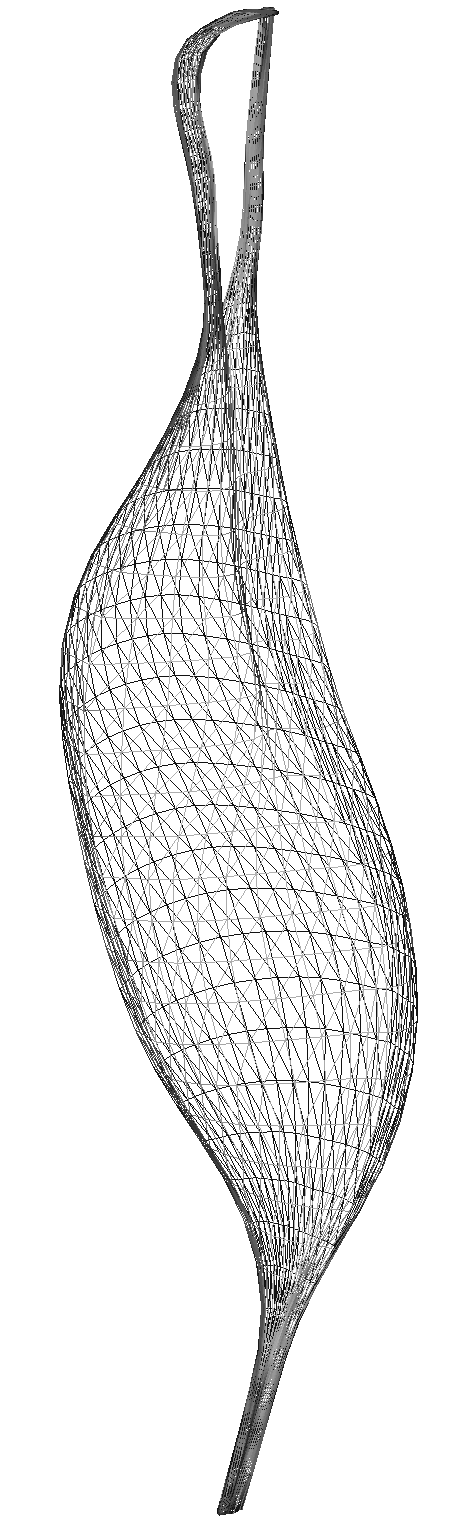
\includegraphics[height=10cm]{images/fiber_creation/biceps22.png}%
  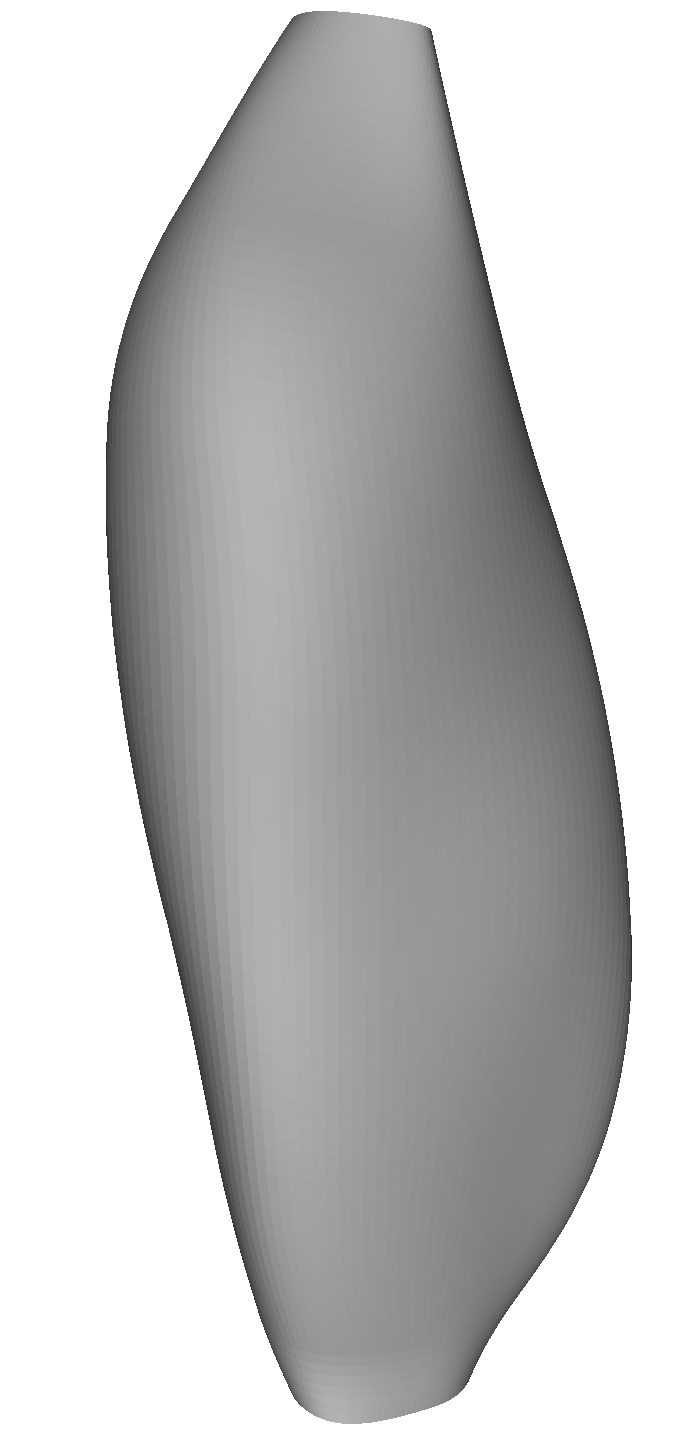
\includegraphics[height=10cm,trim=-2cm 0 0 -2cm, clip]{images/fiber_creation/splines00.png}%
  \caption{Processing the geometry of the biceps brachii muscle. From left to right: mesh with cubic Hermite elements, STL mesh with inside triangles, STL surface mesh where triangles lying inside have been removed, Spline surface of the muscle belly.}%
  \label{fig:biceps_processing}%
\end{figure}%

The Hermite elements can be triangulated and stored as an STL file using the tool \code{cmgui}. This process triangulates the non-planar faces of all Hermite elements. This leads to a dataset with triangles on the surface and in the inside of the volume, as can be seen in the second image of \cref{fig:biceps_processing}. At this stage, the use of the MAP and OpenCMISS related tools is finished and further processing steps are performed using tools from opendihu that we developed on our own.

A Python script removes the triangles in the inside of the volume. The detection whether a triangle is inside the volume is done by casting four rays from the center of gravity of the triangle and determining if the rays intersect any other triangles. The rays have directions $(x,y,z) = (\pm1,\pm1,\frac13)$, where the $z$ axis is oriented along the muscle and the $x$ and $y$ are oriented in radial direction. The ray-triangle intersection is done using the fast Möller-Trumbore algorithm \cite{ray-triangle}. For every ray, all triangles are checked.
Only if all four rays intersect at least one more triangle, the starting triangle is considered to be inside the volume and subsequently removed from the dataset. 

This algorithm has a quadratic time complexity $\O(n^2)$ in the number of triangles $n$. It could be improved by organizing the triangles in a spatially adaptive data structure, such as an octree. Since this preprocessing step has to be performed only once for a given geometry the runtime is not a concern and there is no need for such optimization.

The result of this operation is a triangulated surface, shown in the third image of \cref{fig:scheme_preprocessing}. The next step is to create a Spline surface of the muscle belly, as shown in the right-most image of \cref{fig:scheme_preprocessing}. This is described in the next section.

\subsection{Fitting a Spline surface}\label{sec:nurbs}
The surface representation of the muscle could be obtain from either the left or the right branch of the preprocessing workflow in \cref{fig:scheme_preprocessing}. The surface is given by a point cloud or a number of triangles. To remedy eventual outliers or unphysiological sharp edges from the segmentation, a Spline surface is fitted to the data. This leads to a smooth surface representation and later to a better conditioned Finite Element mesh in the simulation. However, this step is optional. It is also possible to use the surface triangulation from previous section \ref{sec:surf_extr} for the meshing algorithm in the next section \ref{sec:ser_alg_meshes}.

Nonuniform rational B-Splines (NURBS) are used for the surface. A NURBS surface is a generalization of a B-Spline surface. From a modeling point of view, B-spline surfaces have three advantages. First, the B-spline surface can be constructed with given smoothness properties.  Second, the definition of a particular B-spline surface builds on geometric information, which simplifies their creation. More specifically a control polygon mesh in the 3D space is defined. Its convex hull is guaranteed to contain the surface. Third, the geometric parameters of a B-spline surface have only local impacts on the shape of the surface. This allows a B-spline surface of a fixed, low polynomical degree to approximate point clouds with any number of points without loosing approximation quality.

A limitation of B-spline surfaces is that circular and spherical shapes cannot be represented. This limitation is overcome by NURBS surfaces. NURBS surfaces are defined as the perspective projection into 3D space of a B-spline surface in 4D space.

The mathematical description is given in this section, following the notation of \cite{piegl2012nurbs}. The building blocks are the B-spline basis functions of polynomial degree $p$. Given a knot vector 
%
\begin{align*}
  \Xi = (\xi_1, \xi_2, \dots, \xi_k), \quad \text{with } a=\xi_1 \leq \xi_2 \leq \cdots \leq \xi_k = b,
\end{align*}
%
the $i$th B-spline basis function $N_{i,n}$ of degree $n$ is defined recursively starting with the piecewise constant function $N_{i,0}$ for $n=0$,
%
\begin{align*}
  N_{i,0}(\xi) = \begin{cases} 
    1 \, &\xi_i \leq \xi < \xi_{i+1},\\[2mm]
    0 &\text{else},
  \end{cases}
\end{align*}
and using the following relation to define the functions of higher degree, $n > 0$,
\begin{align*}
  N_{i,n}(\xi) = \dfrac{\xi - \xi_i}{\xi_{i+n} - \xi_i} N_{i,n-1}(\xi) + \dfrac{\xi_{i+n+1} - \xi}{\xi_{i+n+1} - \xi_{i+1}} N_{i+1,n-1}(\xi), \quad i > 0.
\end{align*}
Because neighbouring entries in the knot vector can be equal, the fraction $0/0$ can occur. In this case, $0/0 := 0$ is defined.

A B-spline curve $\bfC \in \R^d$ of polynomial degree $p$ is defined as
%
\begin{align*}
  \bfC(u) = \s{i=1}{l}N_{i,p}(u)\,\bfP_i, \quad u \in [a,b].
\end{align*}
%
The coefficients $\bfP_i \in \R^d, i=1, \dots, l$ to the basis functions $N_{i,p}$ are called \emph{control points} and define the control polygon. The number $l$ of basis functions and control points is determined from the number of knots $k$ in an open knot vector and the polynomial degree $p$ as $l = k-p-1$.

The number of equal entries in series in the knot vector is the \emph{multiplicity} of the respective knot value. Usually \emph{open} knot vectors $\Xi$ are used where the first and the last knot occur with a multiplicity of $p+1$.
This make the first and last points of the B-spline curve coincide with the control polygon, $\bfC(a) = \bfP_1$ and $\bfC(b) = \bfP_l$.

The multiplicities of the knots in the knot vector encode information about the smoothness of the B-spline curve. If the knot value $\hat{\xi}$ has a multiplicity of $m$, the B-spline curve will be $p-m$ times continuously differentiable at $\C(\hat{\xi})$.
% This can be seen from the fact that there exist $m$ basis functions with a support that begins at $\hat{\xi}$.

An exemplary B-spline curve is shown in \cref{fig:bspline_curve}. It uses a \emph{non-uniform} knot vector for polynomial degree $p=3$, where the differences between neighbouring knot values $\xi_{i+m} - \xi_i$ vary. The effect of different multiplicities can be seen. $m=p=3$ places the knot on the respective control point, as for $\xi=49$ in the example. $m=p-1=2$ places the knot on the control polygon, as in the example at $\xi=10$. A lower multiplicity $m < p-1$ does not yield to a higher smoothness and in turn does not force the curve on the control polygon. It can also be seen that the B-spline curve stays inside the convex hull of the control polygon which is a property of all B-spline curves \cite{piegl2012nurbs}.
%
\begin{figure}%
  \centering%
  \def\svgwidth{8cm}%
  \input{images/fiber_creation/bspline_curve.pdf_tex}%
  \caption{Exemplary B-spline curve (red) of degree $p=3$ for the knot vector $\Xi = (0,0,0,0,7,10,10,49,49,49,50,50,50,50)$, control points (blue) and control polygon (black).
  Positions of the curve $\bfC(\xi_i)$ at the knots $\xi_i$ are indicated by the red squares and the knot value $\xi$ and its multiplicity $m$ is given. The effect of moving one control point is shown in green.}%
  \label{fig:bspline_curve}%
\end{figure}%
%
The effect of moving one of the 10 control points is visualized with green color in the \cref{fig:bspline_curve}.
The B-spline basis function $N_{i,p}$ has a local support of $S=(\xi_i,\xi_{i+p+1})$. Consequently, only the corresponding part of the curve, $\bfC(\xi)$ for $\xi \in S$ changes.

A B-spline surface is given as tensor product of two B-spline curves:
\begin{equation}\label{eq:bspline_surface}
  \begin{array}{lll}
    \bfS(u,v) = \s{i=1}{l^{(1)}}\s{j=1}{l^{(2)}} N^{(1)}_{i,p^{(1)}}(u)\,N^{(2)}_{j,p^{(2)}}(v)\, \bfP_{i,j},
  \end{array}
\end{equation}
with two polynomial degrees $p^{(1)},p^{(2)}$, ansatz functions $N^{(1)}, N^{(2)}$, numbers of ansatz functions $l^{(1)}, l^{(2)}$ and corresponding knot vectors.

For NURBS, B-spline curves and surfaces are formulated using \emph{homogeneous coordinates}. Every point in Cartesian coordinates $(x,y,z) \in \R^3$ has a set of homogeneous coordinates $(\tilde{x},\tilde{y},\tilde{z},w)=(x\,w,y\,w,z\,w,w)$. Thus, the Cartesian coordinates can be obtain by the \emph{perspective division}, i.e. dividing all but the last coordinate by the weight $w$.

A NURBS surface is given by the same definition as the B-spline surface in \cref{eq:bspline_surface} except that the control points $\bfP_{i,j} \in \R^3$ are enriched with scalar weights $w_{i,j}$ and, thus, replaced by $(\bfP_{i,j}, w_{i,j}) \in \R^4$. The resulting surface $\bfS$ is given in homogenous coordinates. Executing the perspective division yields the form:
%
\begin{align*}
  &\bfT(u,v) = \s{i=1}{l^{(1)}}\s{j=1}{l^{(2)}} R_{i,j}(u,v) \,\bfP_{i,j},\\[4mm]
  &\text{with } R_{i,j}(u,v) = \dfrac{N_{i,p^{(1)}}(u)\,N_{j,p^{(2)}}(v)\,w_{i,j}}{\s{r=1}{l^{(1)}}\s{s=1}{l^{(2)}} N_{r,p^{(1)}}(u)\,N_{s,p^{(2)}}(v)\,w_{r,s}}.
\end{align*}
The new rational basis functions $R_{i,j}$ and the possibly non-uniform knot vectors give rise to the name non-uniform rational B-spline surface.

In order to find a NURBS surface for the given triangulated surface of a muscle, at first, the part of the geometry corresponding to the tendons is removed) such that the resulting triangles model only the muscle belly. The belly has a length of \SI{12.8}{\mm}.

Then, twelve cross sections are extracted from the surface triangles. The result are twelve horizontal circumference rings. On each ring 9 equidistant points are sampled. The first point is appended after the last point in every ring, such that in total we obtain a grid of $10 \times 12$ points. The least squares surface approximation algorithm by \cite{piegl2012nurbs} is used to fit a NURBS surface to the points. The implementation of the algorithm is given by the NURBS-Python (geomdl) library. Polynomial degrees of $p^{(1)} = 3$ and $p^{(2)}=2$ are used where the first dimension corresponds to the cross-sectional direction of the muscle. The knot multiplicity is chosen as $m=1$ for both coordinate directions to obtain a two times respective one times continuously differentiable surface in $u$ and $v$ direction. The resulting NURBS surface and the control polygon is visualized in \cref{fig:biceps_splines_control_points}. Note that the control polygon is different from the grid of points against which the surface is fitted.
%
\begin{figure}%
  \centering%
  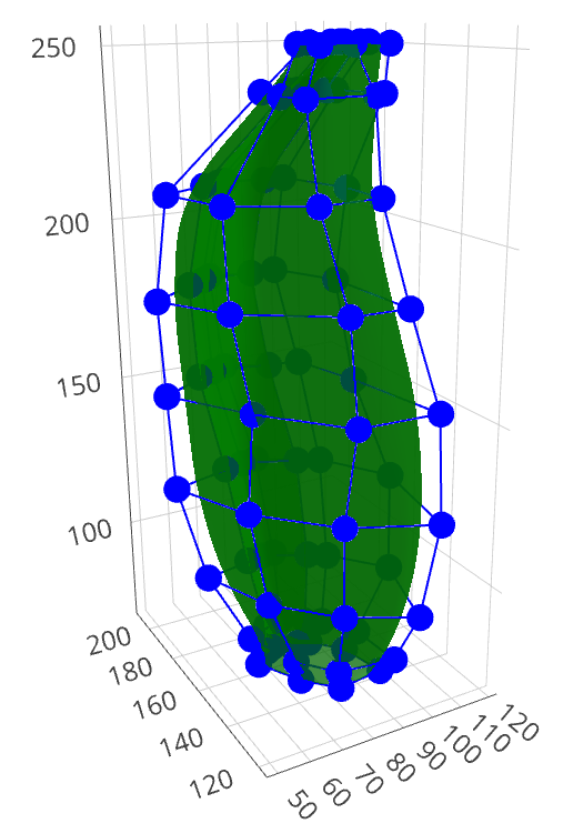
\includegraphics[width=0.35\textwidth]{images/fiber_creation/splines01.png}%
  \caption{Fitted NURBS surface of the biceps muscle (green) and the control polygon (blue).}%
  \label{fig:biceps_splines_control_points}%
\end{figure}%
%
\Cref{fig:biceps_splines_wrong} shows the result of this approach. It can be seen the surface is non-differentiable and has a kink at the seam line where the first and last points of each ring meet. The reason is that the surface fitting algorithm does not pose any conditions on the tangents at the edges of the fitted NURBS surface. Since no implementation of a fitting algorithm specifically for a tubular NURBS surface is available, the point grid is modified. The series of 9 equidistant points on each ring is replicated twice and the first point is again added as the last point. This leads to a grid of $(3\cdot 9+1) = 28 \times 12$ points which wraps around the muscle volume three times. The fitting algorithm is executed on this grid. The resulting NURBS surface also wraps around the muscle three times with the two ends being again not properly fitting to each other. From these three wraps, the middle one is extracted. This corresponds to restricting the NURBS surface $\bfT(u,v)$ from $(u,v) \in [0,1]^2$ to $(u,v) \in [0.4,0.733]\times [0.1]$.

The result is depicted in \cref{fig:biceps_splines_seam} and it can be seen that the tangents now match very well between the two sides of the NURBS surface. Furthermore, the comparison with the inital approach in \cref{fig:biceps_splines_wrong} shows that an artifical bulge at the top of the muscle in the perspective of the visualization is removed. The overall shape of the muscle now looks smoother and more natural. Also in comparison with the result of the automatic algorithm in \cref{fig:extraction_result_biceps}, the results of this approach are smoother.

The generated tubular surface has two holes at the top and bottom which prevent it from being an enclosing surface to the muscle belly volume. The borders of these holes each lie in a plane and, thus, the missing surface is treated as being planar when the 3D meshes are created.
%
\begin{figure}%
  \centering%
  \begin{subfigure}[t]{0.48\textwidth}%
    \centering%
    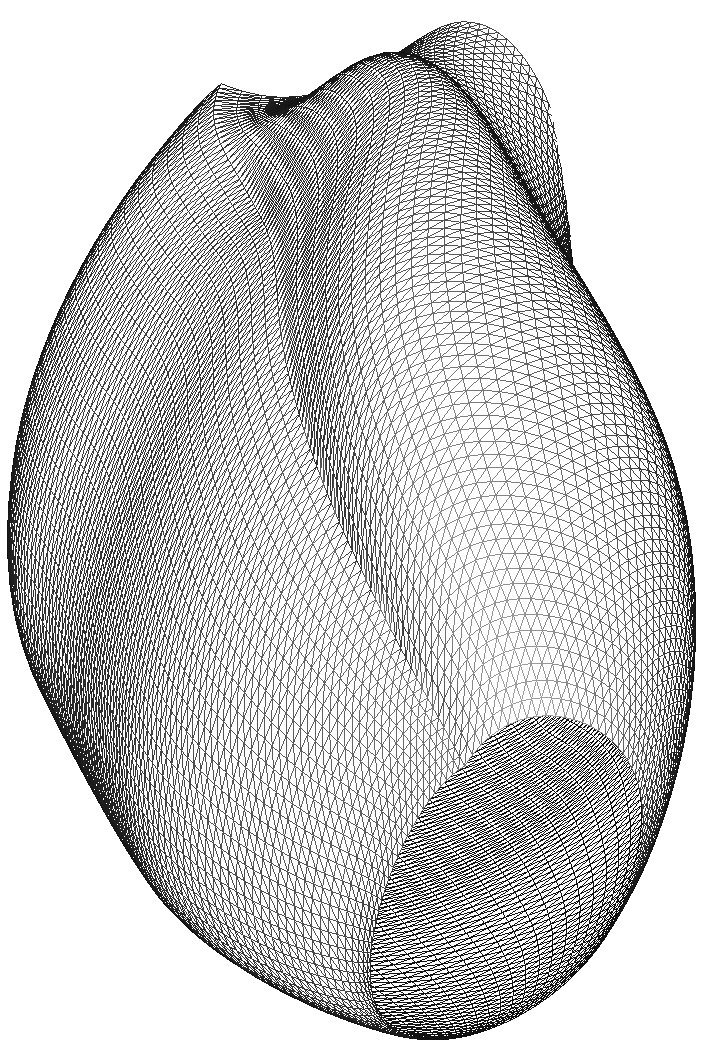
\includegraphics[height=8cm]{images/fiber_creation/splines_wrong00.png}%
    \caption{First approach with $10 \times 12$ points. The kink at the seam line along the muscle is clearly visible.}%
    \label{fig:biceps_splines_wrong}%
  \end{subfigure}
  \quad
  \begin{subfigure}[t]{0.48\textwidth}%
    \centering%
    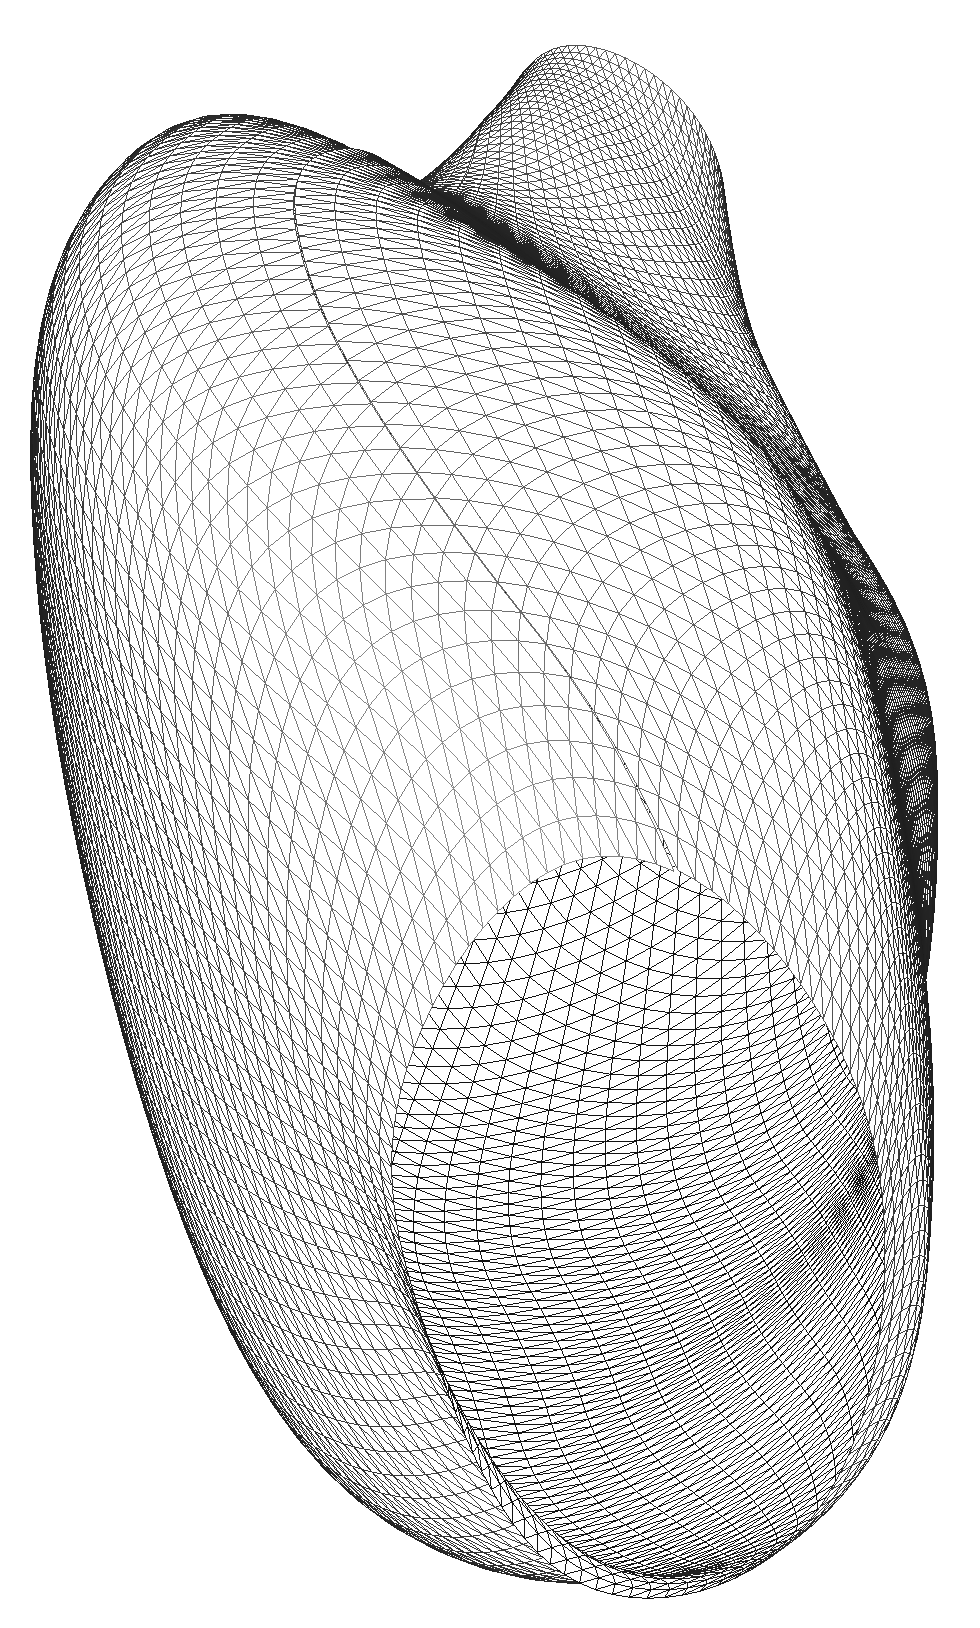
\includegraphics[height=8cm]{images/fiber_creation/splines_seam00.png}%
    \caption{Second, improved approach with $28 \times 12$ points. It can be seen that the tangent at the seam line matches very well.}%
    \label{fig:biceps_splines_seam}%
  \end{subfigure}
  \caption{Fitted NURBS surface of the biceps muscle, triangulated for visualization purposes.}%
  \label{fig:biceps_splines}%
\end{figure}%
%
\section{Serial Algorithm to Create Muscle and Fiber Meshes}\label{sec:ser_alg_meshes}
Next, a 3D mesh for the muscle volume and 1D meshes for muscle fibers need to be generated from the surface representation described in the last sections. In this section, first an algorithm for the 3D mesh is described. Then, a second algorithm that reuses results from the first algorithm is presented which generated one dimensional meshes for muscle fibers. Both algorithms are executed in serial. A derived algorithm that can run in parallel and, thus, on a distributed memory hardware can handle larger datasets is given in the next section, \cref{sec:parallel_algorithm}.

The serial algorithm for generation of the 3D mesh is presented in \cref{alg:serial_algorithm_1} and the steps visualized in \cref{alg:serial_algorithm_1}. Input is the set of triangles at the tubular surface of the muscle. The tubular surface is oriented along the $z$ axis. In the following descriptions the muscle in considered to be oriented upright such that $z$ axis points in vertical direction towards the top. The borders at bottom and top have a constant $z$ coordinate.
%
\begin{algorithm}
  \begin{algorithmic}[1]%
    \Procedure{Create\_3D\_mesh}{}
    \Require triangulated tubular surface
    \Ensure structured 3D volume mesh
    \Statex
    \State Slice geometry           \label{alg:1.1}
    \State Triangulate 2D slices      \label{alg:1.2}
    \State Compute harmonic maps $u, v$      \label{alg:1.3}
    \State Construct regular grid in parameter space and map to slices            \label{alg:1.4}
    \State Form 3D quadrilateral elements between the 2D slices’ meshes   \label{alg:1.5}
    \EndProcedure
  \end{algorithmic}%
  \caption{Serial algorithm}%
  \label{alg:serial_algorithm_1}%
\end{algorithm}%

\subsection{Slicing of the geometry}
The first step in line \algref{alg:serial_algorithm_1}{alg:1.1} states to slice the geometry. This means that horizontal \say{slices} of the cross-sectional area are extracted from the surface mesh. First, the muscle is divided into equidistant positions $z_i, i=1,\dots,n$ along the $z$-axis where the slices are to be extracted. As can be seen in \cref{fig:serial_alg_0}, $n=13$ $z$ coordinates are selected. Next, for every position $z_i$, all surface triangles $T_j$ that intersect the plane $Z_i = \{\bfp=(x,y,z) | z=z_i$\} are considered and the intersection lines $P = T_j \cap Z_i$ are computed. The method of computing plane-triangle intersection is described in the following.

Given is a triangle $T$ with points $\bfp^{1},\bfp^2,\bfp^3 ∈ \R^3$ and a value $\hat{z}$, the wanted result is the set of points $P = T ∩ \{\bfp = (\bfp_x,\bfp_y,\bfp_z) \mid \bfp_z=\hat{z}\}$ which corresponds to a line segment $\overline{\bfp^a\bfp^b}$. 

We describe the points in the triangle by two barycentric coordinates $\xi_1$ and $\xi_2$ as
\begin{equation}\label{eq:barycentric_triangle}
  \begin{array}{lll}
    \bfp(ξ_1,ξ_2) = (1-ξ_1-ξ_2)\,\bfp^{1} + \xi_1\,\bfp^{2} + \xi_2\,\bfp^{3},  \\[4mm]
    \text{with }\xi_1+\xi_2 \leq 1, \quad 0 \leq \xi_1,\xi_2 \leq 1.
  \end{array}
\end{equation}
By letting $\bfp_z(ξ_1,ξ_2) = \hat{z}$ we calculate the equation for the line segment $\overline{\bfp^a\bfp^b}$ in barycentric coordinates to be
\begin{equation*}
  \begin{array}{lll}
    ξ_1 = m\cdot ξ_2 + c,\quad
    m = -\dfrac{\bfp_z^{3} - \bfp_z^{1}}{\bfp_z^{2} - \bfp_z^{1}}, \quad c = \dfrac{\hat{z} - \bfp_z^{1}}{\bfp_z^{2} - \bfp_z^{1}}, \quad \bfp_z^2 \neq \bfp_z^1.
  \end{array}
\end{equation*}
For $\bfp_z^1 = \bfp_z^2 \neq \bfp_z^3$ we swap $\bfp_z^2$ and $\bfp_z^3$.

%
%  # x(xi1,xi2) = (1-xi1-xi2)*x^{1} + xi1*x^{2} + xi2*x^{3},  xi1+xi2 <= 1, 0 <= xi1,xi2 <= 1
%  # x_3(xi1,xi2) = z_value  =>  (1-xi1-xi2)*x^{1} + xi1*x^{2} + xi2*x^{3} = z_value
%  #                         =>  xi1*(x^{2} - x^{1})  +  xi2*(x^{3} - x^{1})  =  z_value - x^{1}
%  #                         =>  xi2 = ((z_value - x^{1}) - xi1*(x^{2} - x^{1})) / (x^{3} - x^{1})
%  #                         =>  xi2 = (z_value - x^{1})/(x^{3} - x^{1}) - xi1 * (x^{2} - x^{1})/(x^{3} - x^{1})
%  #                         =>  xi1 = (z_value - x^{1}) / (x^{2} - x^{1})  - xi2 * (x^{3} - x^{1}) / (x^{2} - %x^{1}) 
We consider the three sides $\overline{\bfp^1\bfp^2}, \overline{\bfp^2\bfp^3}$ and $\overline{\bfp^3\bfp^1}$ of the triangles and check which of them is intersected by the $z=\hat{z}$ plane.
\begin{enumerate}
\item On the triangle side $\overline{\bfp^1\bfp^3}$ we have the condition $ξ_2 = 0$ and the side intersects the plane 
at $\bfp(0,-c/m)$ 
iff $0 \leq c \leq 1$. 
\item On the triangle side $\overline{\bfp^1\bfp^2}$, the condition $ξ_1 = 0$ holds and the side intersects the plane 
at $\bfp(c,0)$ 
iff $m\neq 0 \wedge 0 \leq -c/m \leq 1$. 
\item The third triangle side $\overline{\bfp^2\bfp^3}$ is intersected for $ξ_1=(c+m) / (1+m)$
at $\bfp(ξ_1,1-ξ_1)$ 
iff ${m \neq -1 \wedge 0 \leq (c+m)/(1+m) \leq 1}$.
\end{enumerate}
Only if exactly two of these three conditions for intersection of the triangle sides are met, there is an intersecting line segment $\overline{\bfp^a\bfp^b}$ with $\bfp^a \neq \bfp^b$ and the two intersection points $\bfp^a$ and $\bfp^b$ on the triangle sides need to be computed. The case $\bfp^a = \bfp^b$ and the case where two or more of the triangle points are lying on the $z=\hat{z}$ plane are handled separately.

After the presented computations are performed for all planes $Z_i$ and all triangles $T_j$, we have a number of line segments that form a geometric \say{ring} for each $z$ plane. The line segments are ordered according to their adjacency and a counter-clockwise orientation with respect to the $z$ axis is ensured.
The length of each ring is computed. A number $m=16$ of equidistant points is selected on each ring.

Because the selected points on the rings are later used as border points of the volume mesh, their position relative to each other should be in a tidy manner. When viewing the points on the surface in a $x-z$ or $y-z$ projection, they should approximately form a uniform regular grid. With given rings and number $m$ of equidistant points per ring, only the position of one point per ring is not yet fixed. We define a first condition that relates the point positions of two neighbouring rings and a second condition for one point at the bottom-most ring.

The first condition should ensure that the point positions on neighbouring rings are as similar as possible. This is done by minimizing the distance between the one point on every ring that is fixed first.
In the algorithm, the $z$ planes are traversed from bottom to top. The first point $\tilde{p}_{i,0}$ on a ring at $z=z_i$ is determined from the first point $\tilde{p}_{i-1,0}$ of the previous ring at $z=z_{i-1}$ as the one with the minimal distance $|\tilde{p}_{i,0} - \tilde{p}_{i-1,0}|$. Thus, the searched point $\tilde{p}_{i,0}$ has the property that the line between $\tilde{p}_{i,0}$ and $\tilde{p}_{i-1,0}$ and the tangent of the ring are perpendicular.

Given any point $\bfp$ on the ring at $z_i$ and the tangent vector $\bfu$ at this point, we can project the connection vector $\bfv$ from the start point $\tilde{p}_{i-1,0}$ of previous ring to $\bfp$, $\bfv = \tilde{p}_{i-1,0} - \bfp$, onto the tangent $\bfu$. This leads to the plumb foot point $\bfp_0$ by the computation
\begin{equation*}
  \begin{array}{lll}
    \bfp_0 = \bfp + t\,\bfu \quad \text{with }t = \dfrac{\bfv \cdot \bfu}{|\bfu|^2}.
  \end{array}
\end{equation*}
Performing this calculation for every line segment on a ring allows to select the plumb foot $\bfp_0$ with the smallest distance to the start point $\tilde{p}_{i-1,0}$ of the previous ring to be the start point $\tilde{p}_{i,0}$ of the current ring.

With this first condition, all points are fixed relative to each other. The definition of one point, the start point $\tilde{p}_{0,0}$ of the bottom-most ring, is missing. The second condition therefore fixes this point by a prescribed plane $x = \hat{x}$ and selecting $\tilde{p}_{0,0}$ such that its $x$ coordinate lies in this plane. From the (usually two) points that meet this condition, the one with lower $y$ coordinate is selected. The actual value of $\hat{x}$ is determined experimentally such that the resulting point positions are visually uniform. Because of the shape of the biceps muscle, especially the groove where the humerus bone is located, not every value leads to a good result.

The resulting grid of points on the biceps surface is visualized in \cref{fig:serial_alg_0}. It can be seen that every points of the same ring have the same $z$ coordinate. By connecting neighbouring points, a regular grid can be formed. This overall grid in this $x-z$ perspective view has rather vertical connection lines and looks relatively uniform, compared with the gray surface triangulation mesh of the biceps geometry. The spacing between the points is lower at the top and bottom of the muscle because of the smaller circumference at these locations.

%
\begin{figure}%
  \centering%
  \begin{subfigure}[t]{0.48\textwidth}%
    \centering%
    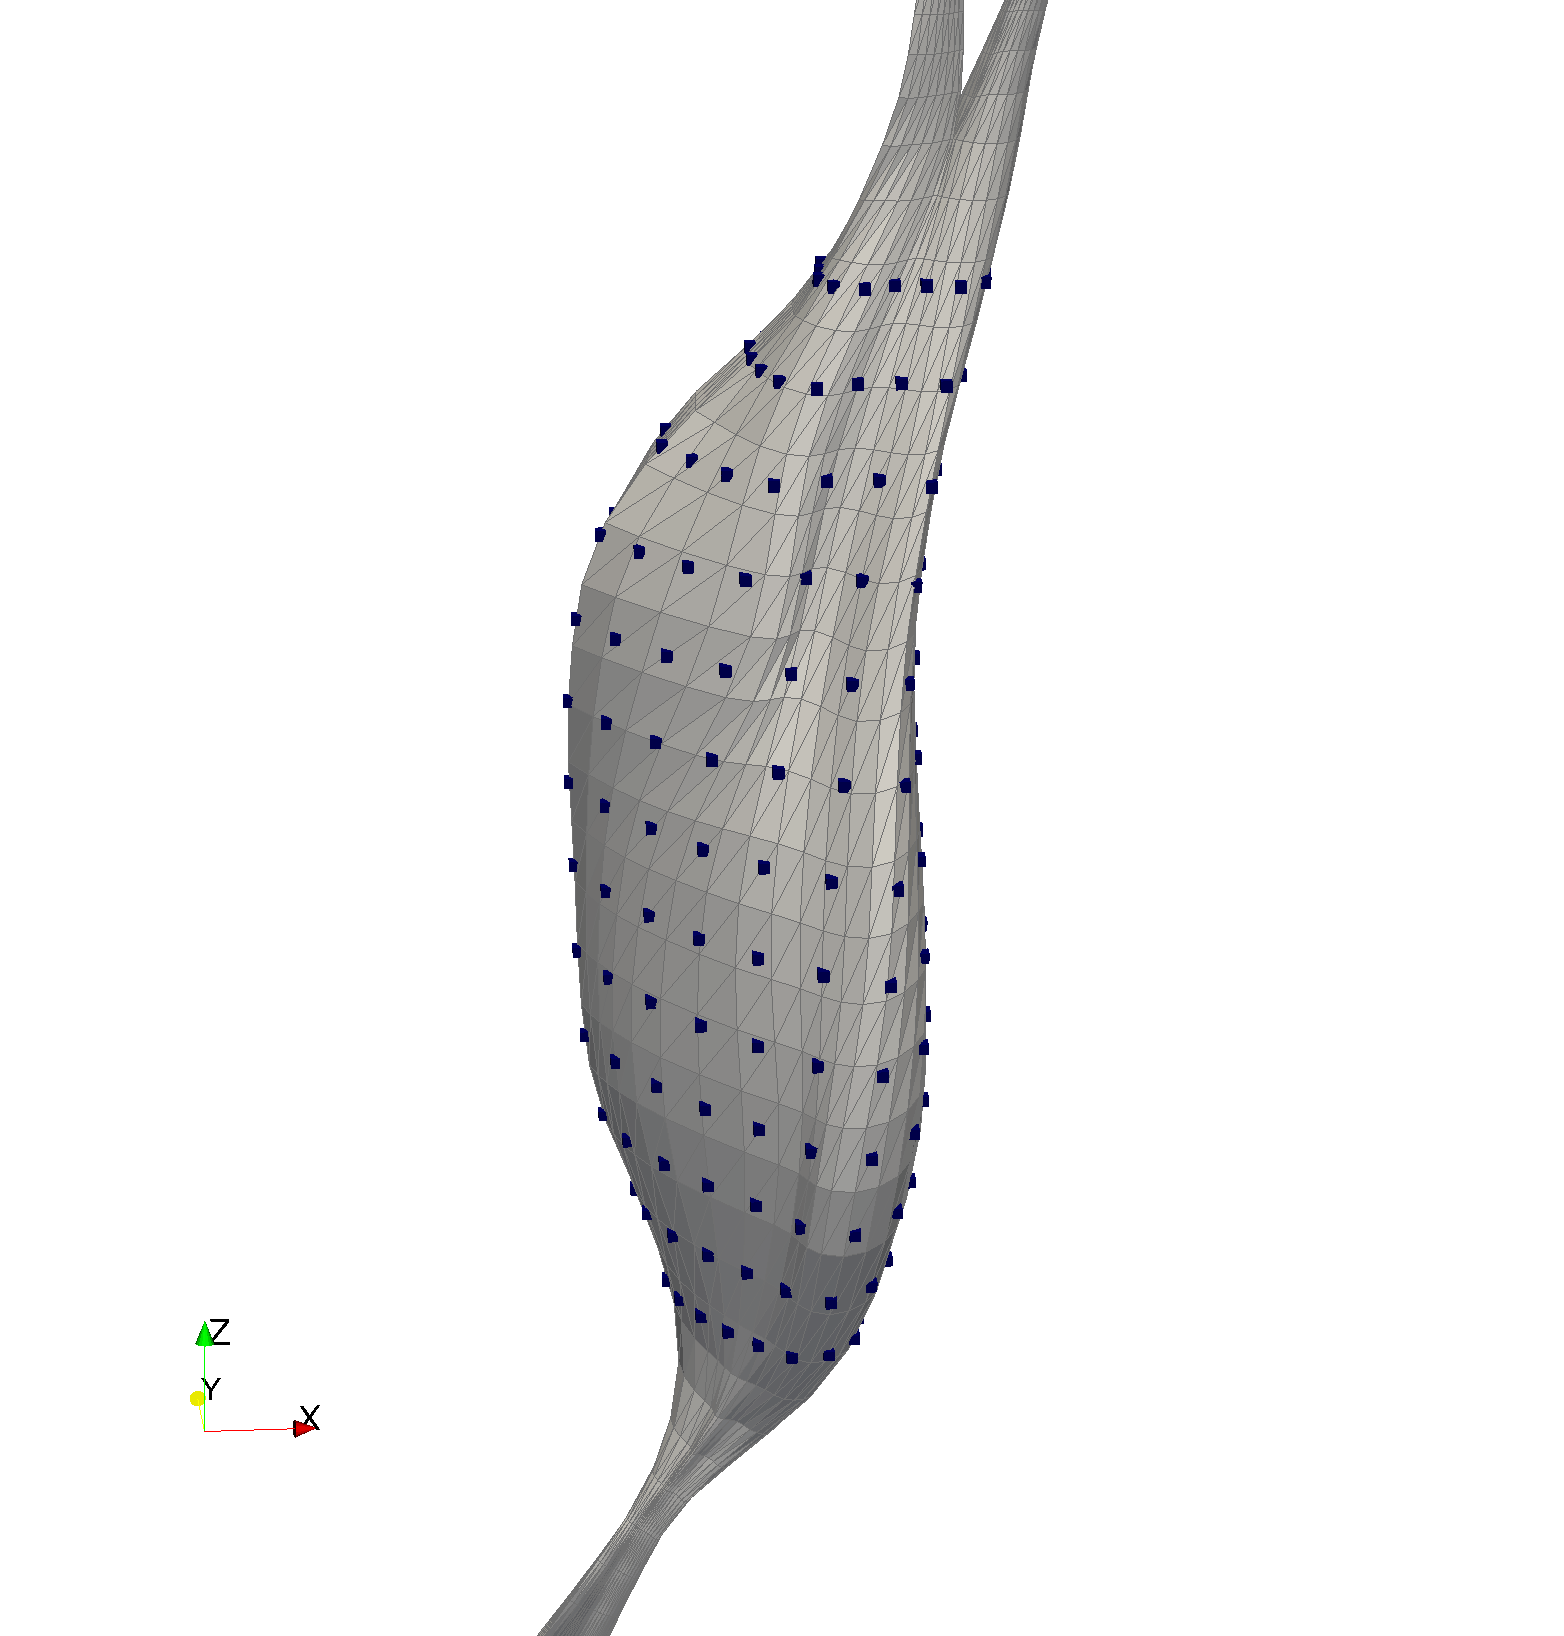
\includegraphics[height=10cm]{images/fiber_creation/serial_alg_0.png}% [trim=left bottom right top, clip]
    \caption{Extracted border points (blue) on the biceps surface mesh (gray). This is the result of line \algref{alg:serial_algorithm_1}{alg:1.1}.}%
    \label{fig:serial_alg_0}%
  \end{subfigure}
  \quad
  \begin{subfigure}[t]{0.48\textwidth}%
    \centering%
    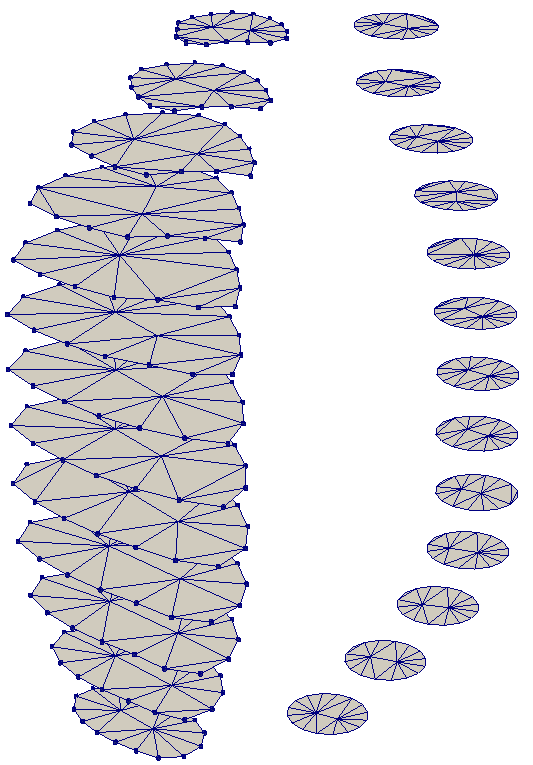
\includegraphics[height=10cm]{images/fiber_creation/serial_alg_3.png}%
    \caption{The generated triangulation of the slices (left) and the image $\bfy(\bfx)$ of the triangulation under the harmonic map (right). This figure shows the result of lines \algref{alg:serial_algorithm_1}{alg:1.2} and \algref{alg:serial_algorithm_1}{alg:1.3}.}%
    \label{fig:serial_alg_3}%
  \end{subfigure}\\
  \centering%
  \begin{subfigure}[t]{0.49\textwidth}%
    \centering%
    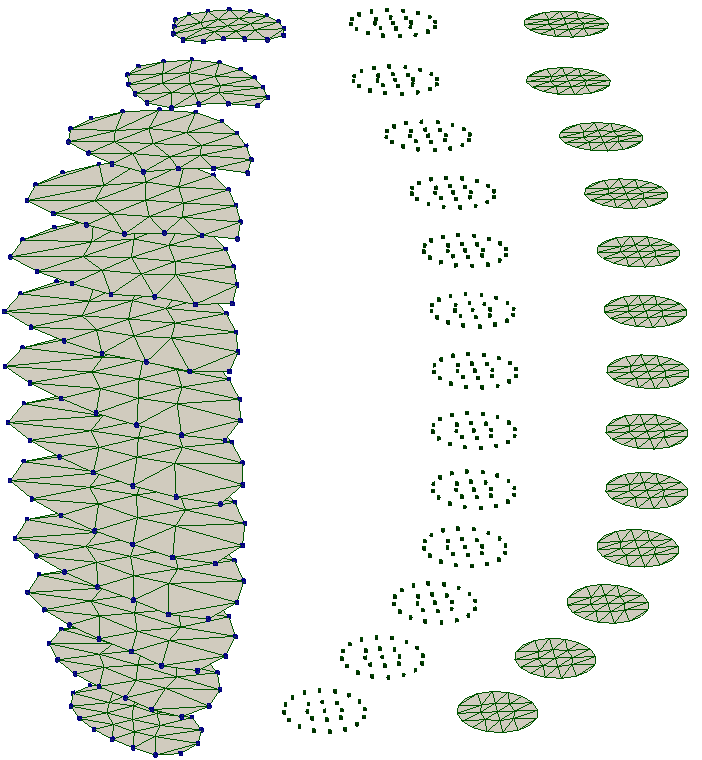
\includegraphics[height=10cm]{images/fiber_creation/serial_alg_4.png}%
    \caption{Grid in parameter space (right) and muscle domain (left), result after line \algref{alg:serial_algorithm_1}{alg:1.4}.}%
    \label{fig:serial_alg_4}%
  \end{subfigure}
  \hfill{}
  \begin{subfigure}[t]{0.4\textwidth}%
    \centering%
    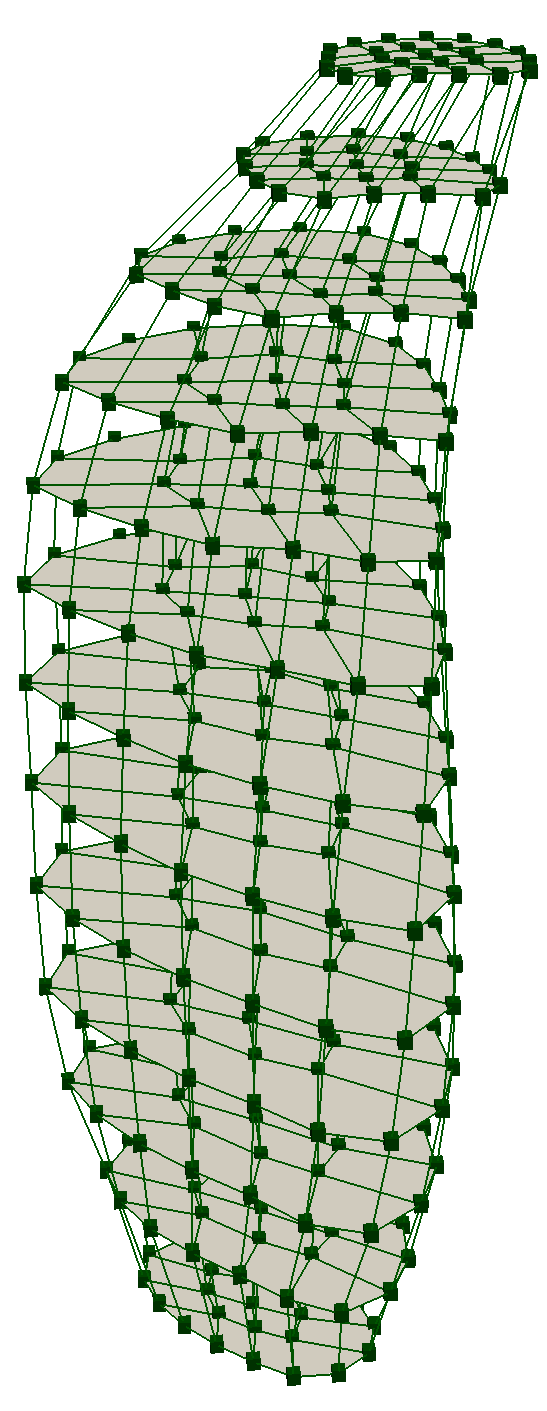
\includegraphics[height=10cm]{images/fiber_creation/serial_alg_8.png}%
    \caption{3D elements formed by connecting the slices, result after line \algref{alg:serial_algorithm_1}{alg:1.5}.}%
    \label{fig:serial_alg_8}%
  \end{subfigure}
  \caption{Steps of the serial algorithm, \cref{alg:serial_algorithm_1}, executed directly on the surface mesh of the biceps muscle (not the B-spline surface).}%
  \label{fig:serial_alg}%
\end{figure}%
%

\subsection{Triangulation of the Slices}\label{sec:triangulation_of_the_slices}
The points of each ring enclose a planar, polygonal surface, a \say{slice} $S_M$ of the muscle.
The next step in the algorithm, line \algref{alg:serial_algorithm_1}{alg:1.2}, is to triangulate the extracted slices, i.e. construct triangles that decompose the polygons. This is visualized at the left side in \cref{fig:serial_alg_3}.

Three different methods have been selected to construct the triangulation. The first and second methods are based on Delaunay triangulations. The third method creates custom triangulation using a simple construction scheme with only one additional point.
\Cref{fig:triangulations} visualizes results of the three methods.

The first method uses the tesselation algorithm from the spatial algorithms and data structures module of the Python package SciPy. 
The Quickhull algorithm \cite{quickhull} is used which triangulates the convex hull of the points. In consequence, the triangulation of concave slices have triangles that lie outside the interior of the slice. An advantage is that the triangulation uses all given points and no new points are added. However, this often results in meshes of lower quality than if adding additional points was allowed.
The example in \cref{fig:triangulation_0} shows a concave slice. At the bottom of the domain, the triangles are outside the slice and almost degenerate.

The second method uses a Delaunay refinement algorithm described in \cite{Delaunay2002} and implementated in the \emph{Triangle} software \cite{shewchuk96b}. A conforming, constrained Delaunay triangulation is created. The triangulation correctly handles convex and concave domains.
Conforming means that the triangulation uses the given points at the border. Additional points at the border as well as in the interior are added. The triangulation is constraint to generate triangles with minimum angles of 20 degrees and a maximum area $A$ that is set to a value dependend on the area of the bounding box. In consequence, all generated triangulations have a guaranteed mesh quality in terms of angles and about the same size and number of triangles.

Comparing the result of the second method in \cref{fig:triangulation_1} with the result of the first method in \cref{fig:triangulation_0} shows the better triangulation quality as the triangles all have higher angles.

The third method places one additional point in the center of gravity of the given points. Triangles are constructed by connecting the center point with two adjacent points on the border, for all given points. The resulting triangulation resembles a pie chart. For some concave slices, this method also creates triangles that partly lie outside the slice. The advantage of this approach is its simplicity.

\Cref{fig:triangulation_2} shows the result for an exemplary slice. Here, in contrast to the first method, the third method creates a valid triangulation despite the concave domain.

\begin{figure}%
  \centering%
  \begin{subfigure}[t]{0.31\textwidth}%
    \centering%
    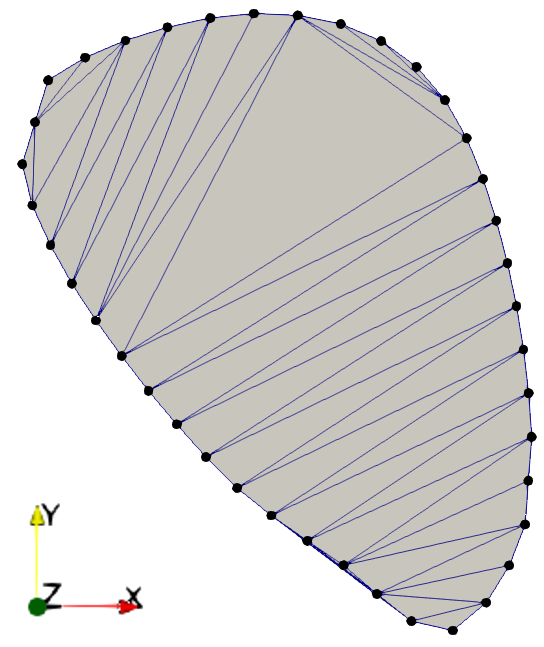
\includegraphics[width=\textwidth]{images/fiber_creation/triangulation_0.png}%
    \caption{First triangulation method}%
    \label{fig:triangulation_0}%
  \end{subfigure}
  \quad
  \begin{subfigure}[t]{0.31\textwidth}%
    \centering%
    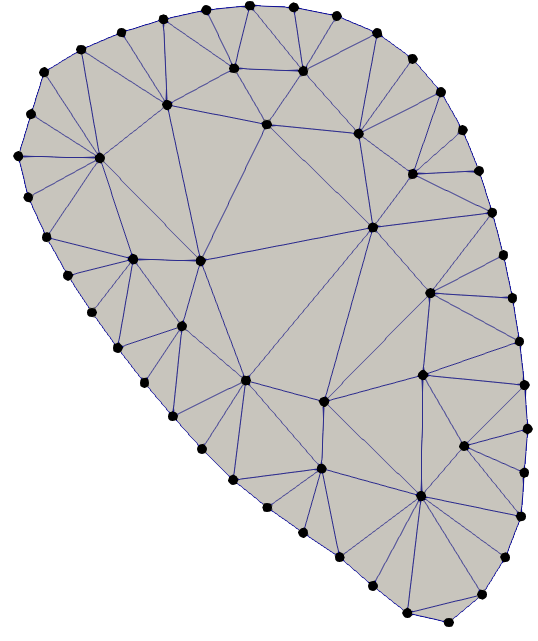
\includegraphics[width=\textwidth]{images/fiber_creation/triangulation_1.png}%
    \caption{Second trian\-gulation method}%
    \label{fig:triangulation_1}%
  \end{subfigure}
  \quad
  \begin{subfigure}[t]{0.31\textwidth}%
    \centering%
    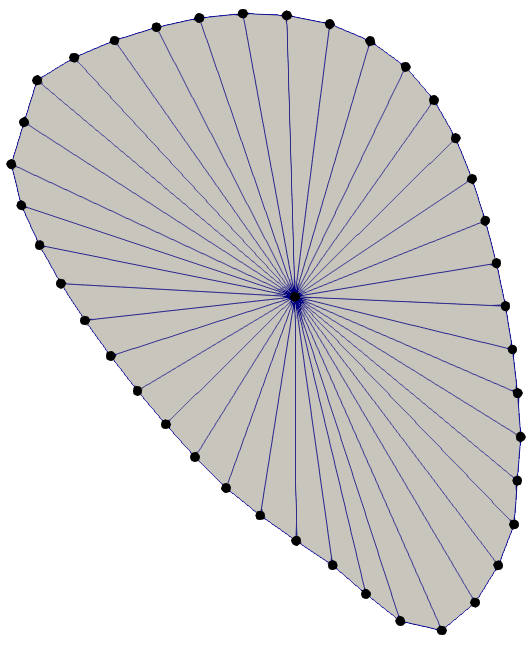
\includegraphics[width=\textwidth]{images/fiber_creation/triangulation_2.png}%
    \caption{Third triangulation method}%
    \label{fig:triangulation_2}%
  \end{subfigure}
  \caption{Result of different triangulation methods for a slice in the center of the biceps muscle.}%
  \label{fig:triangulations}%
\end{figure}%

\subsection{Harmonic Maps}

Next, harmonic maps are created that allow to smoothly map a given 2D reference mesh onto an actual cross-section of the muscle. The initial application of harmonic maps to meshes used for biomedical simulations is given by \cite{marchandise2010quality} and \cite{Marchandise2_2011}. The authors improve a given, oversampled surface mesh obtained from classical segmentation. This is done by partitioning the surface into multiple mesh partitions of zero genus (i.e., containing no holes) and transforming them to a reference space using harmonic maps. There, controlled remeshing is carried out before the transformation is reversed.

In our algorithm, harmonic maps are also used for the purpose of generating high quality meshes. In contrast to the literature, the mapping is based on the muscle slices instead of the surface. Also, different parameter domains are investigated.

In the algorithm, the next step is line \algref{alg:serial_algorithm_1}{alg:1.3}, compute the harmonic maps $u$ and $v$. For a given slice $S_M$, these functions map from $S_M$ to coordinates $u,v\in \R$ of a parameter domain $\Omega_P \subset \R^2$. The parameter domain is either a unit circle or a unit square.

The vector $\bfy(\bfx) := (u(\bfx), v(\bfx))^\top$ for $\bfx \in S_M$ is interpreted as position in $\Omega_P$. The maps are constructed such that the border $∂S_M$ of the slice $S_M$ is evenly mapped to the border $∂\Omega_P$ of the parameter domain $\Omega_P$.
The mapping $\bfy: S_M \to \Omega_P$ is bijective and harmonic, i.e. the Laplace operator of $u$ and $v$ is zero.

More specifically, the definition is
%
\begin{equation}\label{eq:def_harmonic_maps}
  \begin{array}{l}
    u : S_M \to \R, \quad v : S_M \to \R,\\[4mm]
    Δu(\bfy) = 0, \quad Δv(\bfy) = 0 \quad \forall \bfy \in S_M.
  \end{array}
\end{equation}
%
For a uniform parametrization $\bfp:[0,1] \to ∂S_M$ of the border $∂S_M$ of the slice, i.e., 
%
\begin{align*}
  \p{l(t)}{t} = c \in \R \quad \forall t \in [0,1], \quad \text{where } l(t) := \i{0}{t} |\bfp'(\tau)| \,\d\tau,
\end{align*}
%
we require the mapping of the parametrization to be also uniform, i.e.,%
\begin{align*}
  \p{l_P(t)}{t} = c_P \in \R \quad \forall t \in [0,1], \quad \text{where } l_P(t) := \i{0}{t} |\bfy'\big(\bfp(\tau\big)| \,\d\tau.
\end{align*}
%
This leads to the following Dirichlet boundary conditions that close the definition in \cref{eq:def_harmonic_maps}:%
\begin{align}\label{eq:bc_harmonic_maps}
  u(\bfx_\text{M,border}) = u_\text{P,border}, \quad v(\bfx_\text{M,border}) = v_\text{P,border}.
\end{align}
%

\Cref{eq:def_harmonic_maps,eq:def_harmonic_maps} describes a boundary value problem of ordinary differential equations in $u$ and $v$. We solve it using the Finite Element Method and the spatial discretization given by the triangulation of the slices.
Depending on the method of triangulation, a different number of degrees of freedom is given. For the first method with the Quickhull algorithm, no degree of freedom is present and no system of equation needs to be solved. For the third method, only one degree of freedom for the center point needs to be computed. The second method has as many degrees of freedom as there are additional points inserted during the Delaunay refinement.

The first step is to compute the prescribed border points in parameter space,\\
 ${(u_\text{P,border}, v_\text{P,border})^\top}$. When using the first and third triangulation methods, the border points on the slices are  equidistant and therefore the same number of points need to be sampled equidistantly on the border $∂\Omega_P$ of the parameter space.
If the second triangulation method which added additional points is used, also the same number of points  are created on the border $∂\Omega_P$ of the slice as are given on the slice $∂S_M$. The border points are created such that the relations of their distances is the same on $∂\Omega_P$ as for the original points on $∂S_M$.

Using the standard procedure of the Finite Element method for $\nabla u(\bfx) = 0$ on $S_M$ and $u=f(\bfx)$ on $∂S_M$, e.g. as outlined in \cite{Remacle2010}, leads to the weak form with ansatz and test functions $\phi$,
\begin{align}\label{eq:est_fe_w}
    \i{S_M}{} (\nabla u^\top \nabla \phi + \nabla f(\bfx)^\top \nabla \phi) \,\d \bfx = 0 \quad \forall \phi \in \mathcal{H}_0^1.
\end{align}
Standard linear hat functions are used on the triangles with the interpolation property $\phi_i(\bfx_j) = \delta_{ij}$. Using the barycentric parametrization of triangles with points $\bfp^1,\bfp^2$ and $\bfp^3$ introduced in \cref{eq:barycentric_triangle} we get for the ansatz functions and their derivatives within the elements
%
\begin{align*}
  \phi^{(e)}_1 &= (1 - \xi_1)(1 - \xi_2), \quad&
  \phi^{(e)}_2 &= \xi_1 (1 - \xi_2), \quad &
  \phi^{(e)}_3 &= (1 - \xi_1) \xi_2,\\[4mm]
  \nabla \phi^{(e)}_1 &= (\xi_2-1, \xi_1 - 1)^\top, \quad&
  \nabla \phi^{(e)}_2 &= (1-\xi_2, -\xi_1)^\top, \quad&
  \nabla \phi^{(e)}_3 &= (-\xi_2, 1-\xi_1)^\top.
\end{align*}
The superscript $\square^{(e)}$ refers to the definition of the functions within elements. The usual global assembly involves composing the global, nodal functions $\phi_i(\bfx)$ for nodes indexed by $i=1, \dots, n_\text{nodes}$ and using a mapping between the barycentric coordinates $\xi_1,\xi_2 \in [0,1]^2$ inside the elements to the global coordinates $\bfx \in S_M$.

Inserting the discretization
\begin{align*}
  u_h(\bfx) = \s{i=1}{n_\text{nodes}} u_i\,\phi_i(\xi_1(\bfx), \xi_2(\bfx))
\end{align*}
into \cref{eq:est_fe_w} leads to the form
\begin{equation}\label{eq:est_weak_form}
  \begin{array}{lll}
    \s{i=1}{n_\text{nodes}}u_i \i{S_M}{} \nabla_\bfx \phi_i^\top \nabla_\bfx \phi_j \,\d\bfx + \s{i=1}{n_\text{nodes}} f_i \i{S_M}{} \nabla_\bfx \phi_i^\top \nabla_\bfx \phi_j \,\d \bfx = 0\,\quad \forall j=1,\dots,n_\text{nodes}.
  \end{array}
\end{equation}
The integrations are executed element-wise and over the elemental coordinates $\xi_1,\xi_2$. 

The transformation to elemental coordinates involves the computation of the Jacobian $J=\d\bfx/\d\bfxi$ of the mapping between element coordinates $\bfxi = (ξ_1,ξ_2)$ and global coordinates $\bfx$. From the definition \cref{eq:barycentric_triangle} it follows that
\begin{align*}
  J = \d{\bfx}{\bfxi} = [\bfp^2-\bfp^1, \bfp^3-\bfp^1].\\[4mm]
\end{align*}
The metric tensor for this mapping is given by
\begin{align*}
  \mathcal{M} := \left(\d{x}{\bfxi}\right)^T \, \left(\d{x}{\bfxi}\right).
\end{align*}
%
The transformation of the integrals in \cref{eq:est_weak_form} introduces an additional integration factor of $\sqrt{\det{\mathcal{M}}}$.

We get the following matrix equation:
\begin{align}\label{eq:est_fe_system}
  M_u \bfu = -M_f\,\bff,
\end{align}
with the vector $\bfu$ of nodal solution values, the vector $\bff$ of nodal Dirichlet boundary condition values at the border and the global stiffness matrices $M_u$ and $M_f$. The two global stiffness matrices are assembled from the element stiffness matrices $M^\text{el}$ for the degrees of freedom at all nodes respectively at the border nodes. The entries of the element stiffness matrices are given by
\begin{align*}
  M^\text{el}_{i,j} = \i{0}{1}\i{0}{1-\xi_1}   \nabla \phi_i^{(e)}(\xi_1,\xi_2)^\top \, \mathcal{M}^{-1} \, \nabla \phi_j^{(e)}(\xi_1,\xi_2) \, \sqrt{\det{\mathcal{M}}}  \,\d\xi_2\d\xi_1.
\end{align*}
By solving \cref{eq:est_fe_system} for $\bfu$ we get the discretized harmonic map $u$.
The Finite Element formulation and computation for $v$ is analogous and uses the same global stiffness matrices.

\Cref{fig:harmonic_map_solution} visualizes the triangulation of $S_M$ and the solutions $u(\bfx)$ and $v(\bfx)$ in the first two plots. The color range from bright yellow to dark violet corresponds increasing values of $u$ and $v$. It can be seen that the $u$ values increase from left to right whereas the $v$ values increase from bottom to top, corresponding to the horizontal and vertical coordinate axis $y_1$ and $y_2$ of $\Omega_P$.


Applying the computed harmonic map $\bfy(\bfx)$ to the triangulation of the slices results in a triangulation of the parameter domain $\Omega_P$. This is shown in the third plot of \cref{fig:harmonic_map_solution} and in \cref{fig:serial_alg_3}.
The generated triangulation of the slices was generated using the second triangulation method with the constrained Delaunay triangulation. On the right, the image $\bfy(\bfx)$ under the harmonic map of the triangulation in the slices is shown on the unit circle parameter domains.

\begin{figure}%
  \centering%
  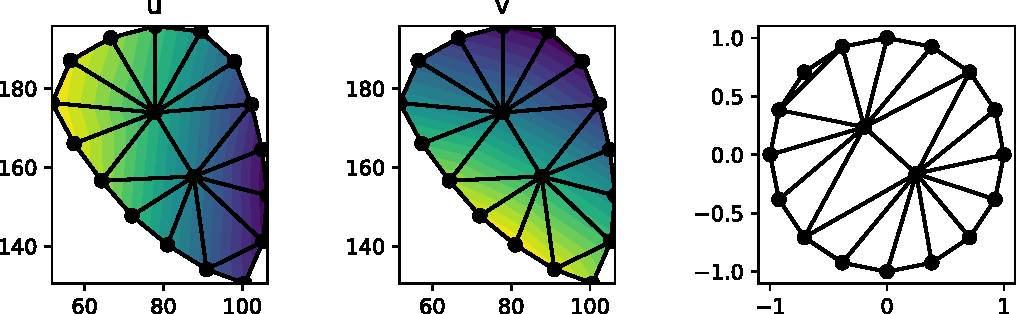
\includegraphics[width=\textwidth]{images/fiber_creation/harmonic_map_9b.pdf}%
  \caption{Triangulations and harmonic map for a slice $S_M$ of the biceps muscle. The first two plots show the solutions of $u$ and $v$ on the slice $S_M$. The third plot shows the image in $\Omega_P$ of the triangulation in $S_M$ under the harmonic map.}%
  \label{fig:harmonic_map_solution}%
\end{figure}%

\subsection{Construction of a regular grid in the parameter domain}
The next step in the \cref{alg:serial_algorithm_1} is the construction of a structured, regular grid in the parameter domain $\Omega_P$, as stated in line \algref{alg:serial_algorithm_1}{alg:1.4}. This grid will then be mapped to the slices $S_M$. Creating a structured grid in a given domain is also called \emph{quadrangulation}.

The parameter domain $\Omega_P$ can be selected to be either a unit square or a unit circle. For both choices, two different schemes how to generate a grid with given number of cells can be selected.
\Cref{fig:quads} shows all four possiblities.

The first scheme, \cref{fig:quad_1}, uses an equidistant regular grid. The grid will be mapped to a cross section of the muscle which has no sharp corners like the unit square. Therefore, the cells of the grid will be distorted at the corners, usually shortening diagonals that point towards the corners and stretching the other diagonals. This assumption motivates the second scheme in \cref{fig:quad_2}. Here, the elements are already distorted in the described manner, with increasing distortion closer to the corners.

A different approach is to use a unit circle, which has no corners and therefore might more resemble a muscle cross section. The first scheme of the unit circle is given in \cref{fig:quad_0}. It uses the radial and circumferential directions for the two dimensions of the grid. A disadvantage of this scheme is that the quadrilaterals at the center are degenerated to triangles. Additionally, the area of the cells varies significantly and the outer cells have unequal side lengths. To remedy this problem, the second scheme given in \cref{fig:quad_3} is constructed. When traversing from the outer border towards the center point and considering the circumferential lines of grid points, the circle morphs into a square as the number of grid points decreases. This approach has the disadvantage that some cells have an inner angle of nearly \SI{180}{\degree}, especially four elements at the border.

Each construction schemes allows to specify the (squared) number of nodes and in consequence the number of cells. The examples in \cref{fig:quad_1,fig:quad_2,fig:quad_3} have $11 \times 11$ nodes and $10 \times 10$ cells. For \cref{fig:quad_0}, the numbers are slightly different. There are $10 \times 11 + 1$ nodes resulting in $10 \times 11$ cells.

\begin{figure}%
  \centering%
  \begin{subfigure}[t]{0.48\textwidth}%
    \centering%
    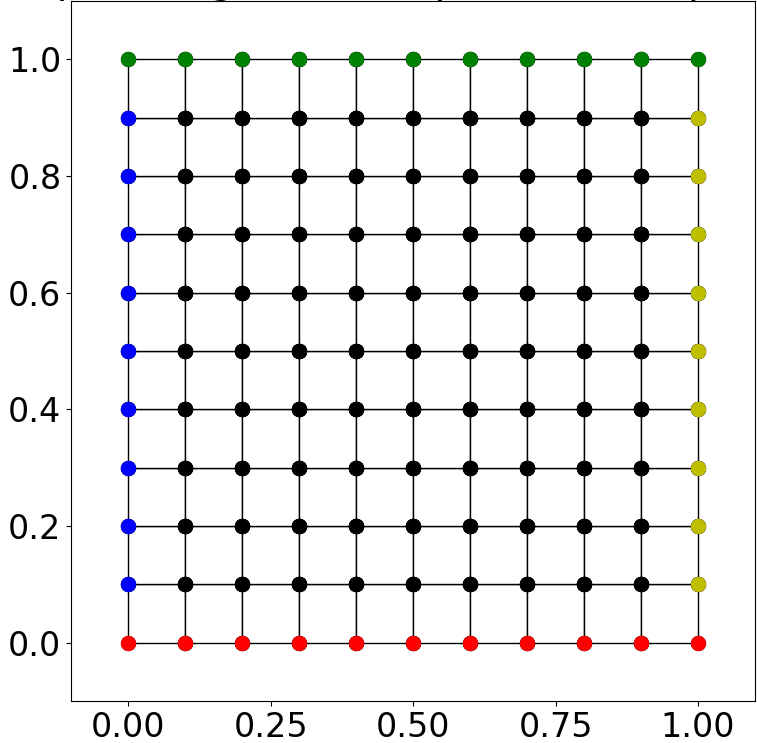
\includegraphics[width=\textwidth]{images/fiber_creation/quad_1.png}%
    \caption{Unit square, scheme 1}%
    \label{fig:quad_1}%
  \end{subfigure}
  \quad
  \begin{subfigure}[t]{0.48\textwidth}%
    \centering%
    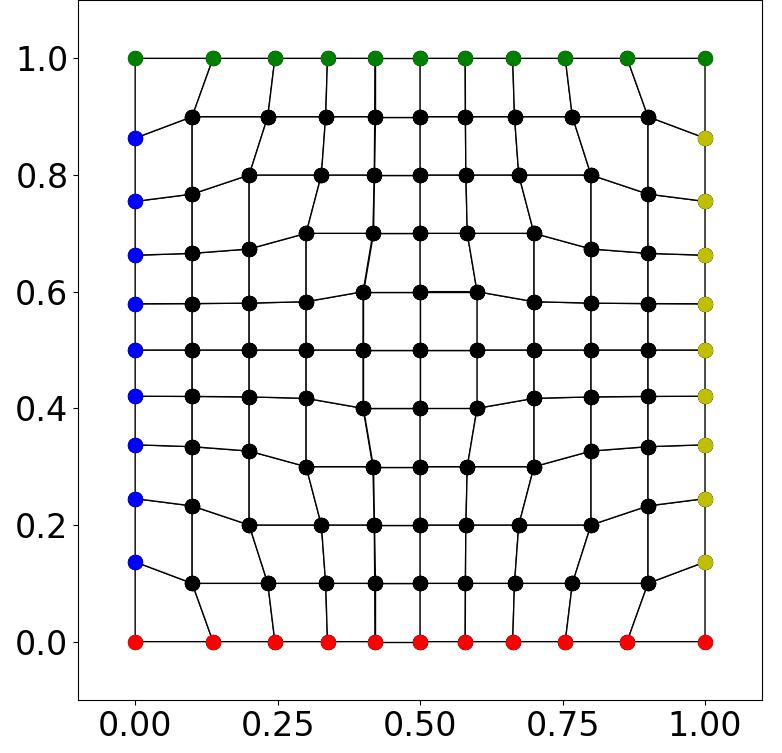
\includegraphics[width=\textwidth]{images/fiber_creation/quad_2.png}%
    \caption{Unit square, scheme 2}%
    \label{fig:quad_2}%
  \end{subfigure}
  \begin{subfigure}[t]{0.48\textwidth}%
    \centering%
    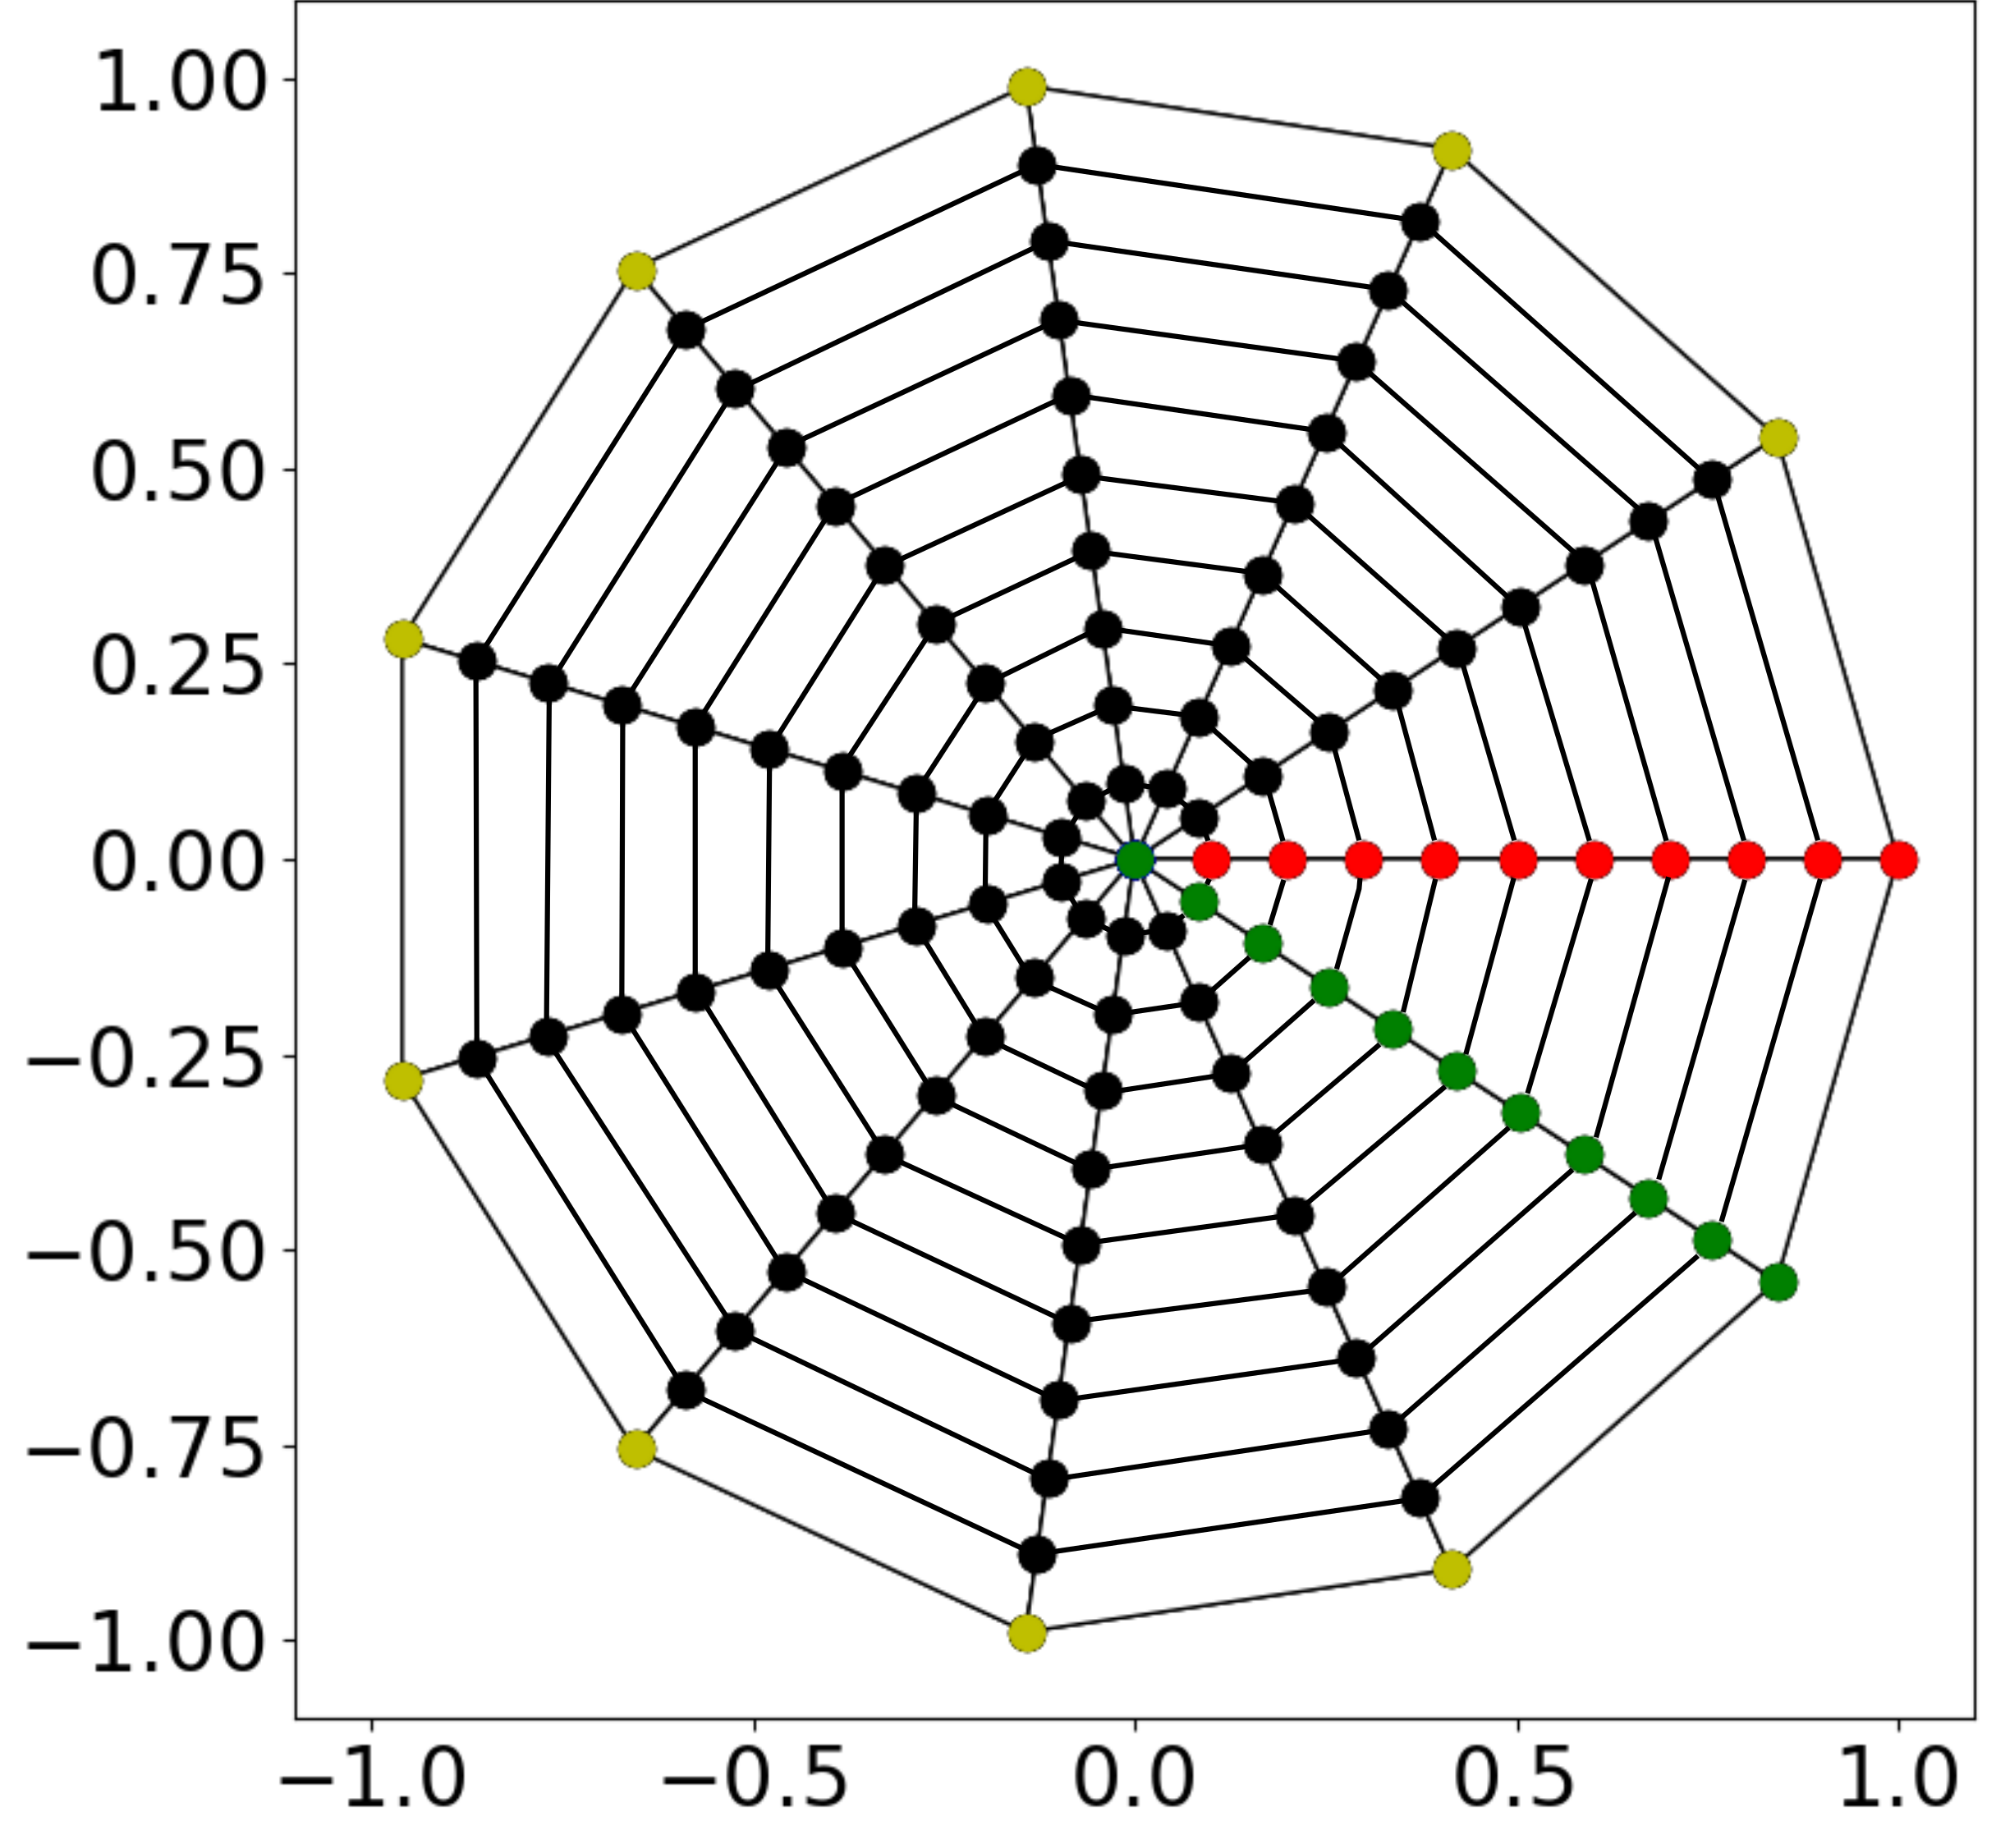
\includegraphics[width=\textwidth]{images/fiber_creation/quad_0.png}%
    \caption{Unit circle, scheme 1}%
    \label{fig:quad_0}%
  \end{subfigure}
  \quad
  \begin{subfigure}[t]{0.48\textwidth}%
    \centering%
    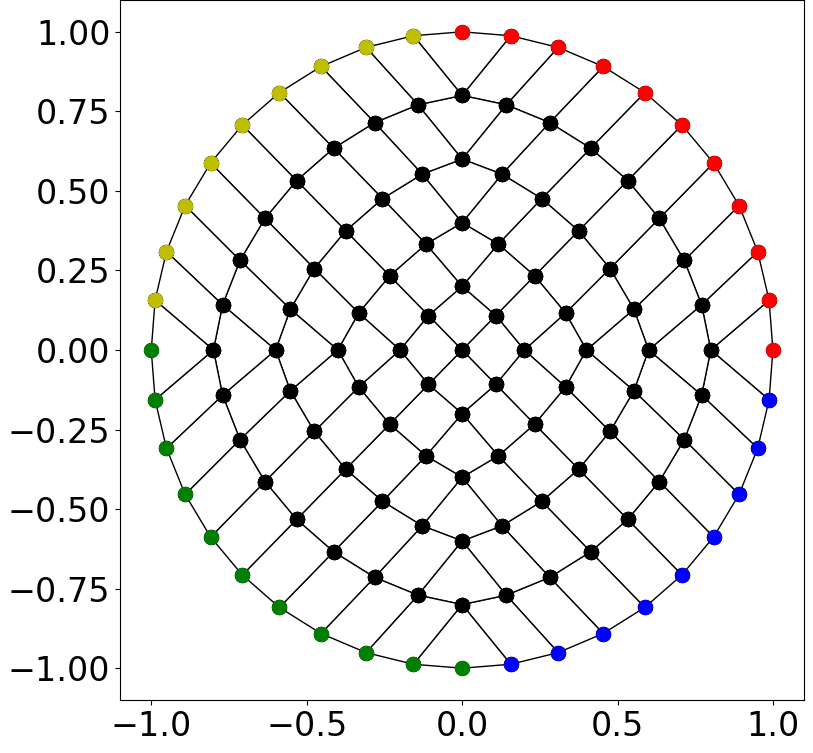
\includegraphics[width=\textwidth]{images/fiber_creation/quad_3.png}%
    \caption{Unit circle, scheme 2}%
    \label{fig:quad_3}%
  \end{subfigure}
  \caption{Different quadrangulation schemes of the parameter domain with $11\times 11$ nodes. The borders of the grid are colored for better perceptiblity.}%
  \label{fig:quads}%
\end{figure}%

Next, the grid in the parameter domain is transferred to the muscle domain by applying the harmonic map $\bfy(\bfx) \in S_M$ on every point of the quadrangulation $\bfx \in \Omega_P$. This is illustrated in \cref{fig:serial_alg_4} for a parameter domain consisting of the unit circle, with quadrangulation scheme 2 and $5 \times 5$ nodes. The cells of the grid in $\Omega_P$ are shown in the right-most stack of domains. The grid points are visualized left of the grids. The resulting image of the mesh in the slices $S_M$ is shown on the left. For visualization reasons, each quadrilateral has been split into two triangles.

\subsection{Formation of Three-Dimensional Elements}

The result of the previous steps is a number of quadrangulated muscle slices. The grid on every slice has the same number of nodes and elements. The nodes on the border of neighbouring slices are positioned similarly.

The final step of \cref{alg:serial_algorithm_1} is line \algref{alg:serial_algorithm_1}{alg:1.5}, the formation of 3D elements. Inserting edges between all corresponding nodes on two neighbouring slices creates a set of 3D elements and, thus, an overall 3D quadrilateral mesh of the muscle volume. This step is visualized in \cref{fig:serial_alg_8}.

\subsection{Generation of Fiber Meshes}

1D fiber meshes are created following the approach of computing a divergence free vector field introduced in \cite{Choi2013}. The steps are given in \cref{alg:serial_algorithm_2}.

The Laplace problem to be solved can be stated as%
\begin{align}\label{eq:fiberest_laplace}
  Δp(\bfx) = 0 \quad \text{for } \bfx \in \Omega_M.
\end{align}
As proposed by \cite{Choi2013}, Neumann boundary conditions can be specified for the bottom and top surfaces of the muscle volume, $∂\Omega_{M, \text{bottom}}$ and $∂\Omega_{M, \text{top}}$:
\begin{align}\label{eq:fiberest_neumann}
  \d{p(\bfx)}{\bfx} \cdot \bfn &= F_\text{in}, \quad &&\text{for } \bfx \in ∂\Omega_{M, \text{bottom}},\\[4mm]
  \d{p(\bfx)}{\bfx} \cdot \bfn &= F_\text{out}, \quad &&\text{for } \bfx \in ∂\Omega_{M, \text{top}}.
\end{align}
The in and outflow values $F_\text{in}, F_\text{out}>0$ are balanced such that the total inflow ${F_\text{in}\cdot \mu(∂\Omega_{M, \text{bottom}})}$ equals the total outflow ${F_\text{in}\cdot \mu(∂\Omega_{M, \text{bottom}})}$. Here, $\mu(∂\Omega)$ is the surface area of the respective boundary.

Alternatively, Dirichlet boundary conditions can be specified:
\begin{align}\label{eq:fiberest_dirichlet}
  p(\bfx) &= 0, \quad &&\text{for } \bfx \in ∂\Omega_{M, \text{bottom}},\\[4mm]
  p(\bfx) &= 1, \quad &&\text{for } \bfx \in ∂\Omega_{M, \text{top}}.
\end{align}
The specification of Dirichlet boundary conditions is easier. Like Neumann boundary conditions, they enforce in and outflows orthogonal to the border.

The boundary value problem given by \cref{eq:fiberest_laplace,eq:fiberest_neumann}  or \cref{eq:fiberest_laplace,eq:fiberest_neumann} is discretized by the Finite Element method with linear or quadratic ansatz functions and solved by \opendihu{} using the 3D mesh generated from \cref{alg:serial_algorithm_1}. The divergence free gradient field is visualized in \cref{fig:potential_flow}. The gradient values are directly given by the Finite Element discretization. The gradient is elementwise constant for linear ansatz functions and trilinear for quadratic ansatz functions.

The next step is line \algref{alg:serial_algorithm_2}{line:2.3} in the algorithm, trace streamline through the gradient field. Seed points are selected at the vertical center of the muscle domain and horizontally at regular subdivisions of the existing 3D elements. Because the 3D mesh was created using harmonic maps, the spacing between the seed points is very uniform.

For the tracing of streamlines, the semi-analytical Pollock's method \cite{Pollock1988} is often used, which was originally developed for fixed 2D finite difference grids. Extensions to irregular 3D grids exist \cite{HAEGLAND2007Streamline}. Other, more accurate algorithms exist \cite{cordes1992continuous}, including higher order formulations \cite{juanes2006unified}.

Because modelling muscle fascicles is only a heuristic approach the generated streamlines do not have to be exceptionally accurate. Therefore, we use a fully numeric method. The streamlines are generated by explicit integration of the gradient vectors in top and bottom direction. A small spatial step width is used. In line \algref{alg:serial_algorithm_2}{line:2.4} all generated streamlines are resampled to obtain the desired widths of the 1D elements.
\Cref{fig:fiber_tracing_streamlines} visualizes the resulting streamlines.

\begin{algorithm}
  \begin{algorithmic}[1]%
    \Statex\Procedure{Create\_1D\_meshes}{}
    \Require structured 3D volume mesh
    \Ensure 1D fiber meshes
    \Statex
    \State Solve Laplacian flow problem   \label{line:2.2}
    \State Trace streamlines in the gradient field  \label{line:2.3}
    \State Resample 1D fiber meshes \label{line:2.4}
    \EndProcedure
  \end{algorithmic}%
  \caption{Serial algorithm}%
  \label{alg:serial_algorithm_2}%
\end{algorithm}%



\begin{figure}%
  \centering%
  \begin{subfigure}[t]{0.48\textwidth}%
    \centering%
    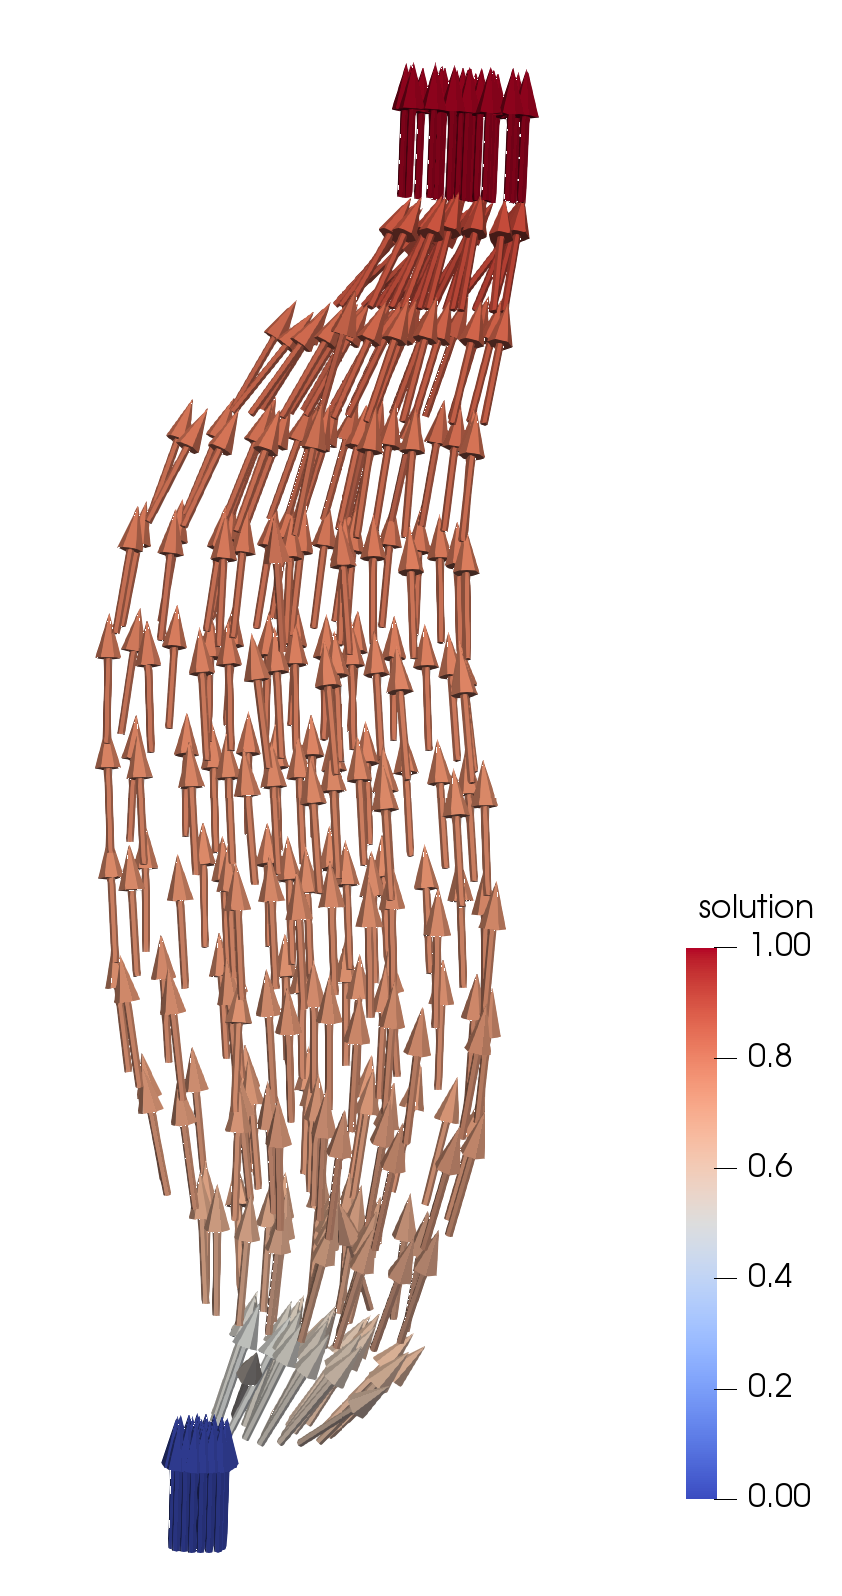
\includegraphics[height=10cm]{images/fiber_creation/potential_flow.png}%
    \caption{Solution (color coding) and direction vectors of the gradient field for the boundary value problem \cref{eq:fiberest_laplace} with Dirichlet boundary conditions \cref{eq:fiberest_dirichlet}.}%
    \label{fig:potential_flow}%
  \end{subfigure}
  \quad
  \begin{subfigure}[t]{0.48\textwidth}%
    \centering%
    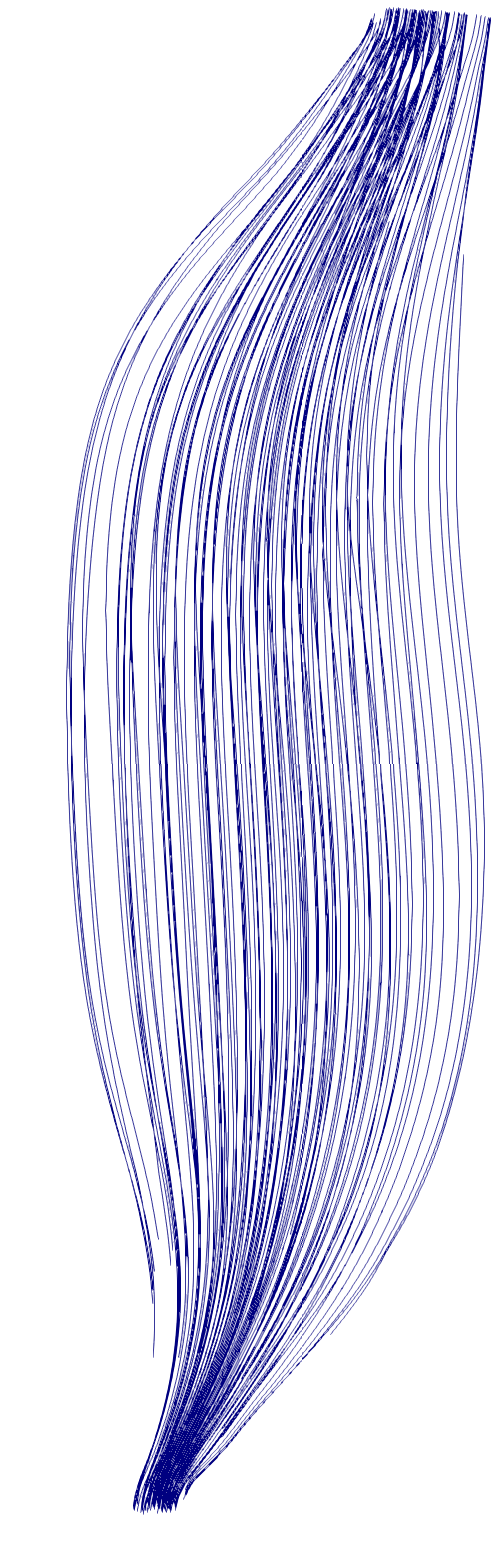
\includegraphics[height=10cm]{images/fiber_creation/streamlines.png}%
    \caption{Resulting streamlines that were traced using the gradient field.}%
    \label{fig:fiber_tracing_streamlines}%
  \end{subfigure}
  \caption{Result of the Laplace problem for the biceps geometry.}%
  \label{fig:potential_flow_streamlines}%
\end{figure}%
%
\subsection{Results and Discussion}
The presented \cref{alg:serial_algorithm_1,alg:serial_algorithm_2} generate a 3D mesh and 1D muscle fibers from a triangulated surface. Different triangulation strategies for the slices and different reference quadrangulations can be chosen. In the following, the different choices are evaluated.

The different triangulation methods for the slices that are discussed in \cref{sec:triangulation_of_the_slices} are visualized in the three columns of \cref{fig:tri_triangulations}. 

The top rows shows the triangulation of $S_M$ and the harmonic map $u$ as color coded value from violet to yellow. $u$ is the horizontal coordinate on the reference domain. A point with violet color in $S_M$ will be mapped to a left-most point in the parameter space $\Omega_P$. Similarly, a yellow point will be mapped to a point far at the right in $\Omega_P$.

The middle and bottom row in \cref{fig:tri_triangulations} show the image of the triangualation under the harmonic map in $\Omega_P$, for the unit square and the unit circle, respectively. The mapping between the colored border points was a prescribed Dirichlet boundary condition in the construction of the harmonic map. It can be seen that the border points are equally spaced both in the muscle domain $S_M$ and in the parameter domain $\Omega_P$.

It can be seen that the triangulation appears distorted in the parameter domains. The effect is highest for the square in the columns \cref{fig:triu_1} and \cref{fig:triu_2}. For the latter the center point of the muscle domain $S_M$ gets mapped far off the center of the squared parameter domain. This effect is hardly visible for the circle.

The reason for this lies in the triangulation of $S_M$ together with its the border shape. In the third method, only the value at the center point is a degree of freedom in the computation of $u$ while the values at the border points are fixed. By the triangulation, the value of $u$ varies linearly from the border to the center point.
By comparing the colored border points with the square in the second row, it can be seen that the prescribed values for $u$ are 0 at all blue points, 1 at all yellow points and linearly increasing from 0 to 1 at the green and red points, increasing from left to right.
The yellow points of $S_M$ with the prescribed constant value of $u=1$ are approximately located on a vertical line. The first two derivatives of $u$ in vertical coordinate direction are therefore almost zero, in consequence, the Laplace equation forces the derivatives in horizontal direction to also be approximately zero. Therefore, the solution value at the center point becomes close to $1$. This leads to the mapped center point being close to the right border in the square parameter domain. The same happens for the vertical coordinate $v$ of the harmonic map.

For the circle, neighboring border points are not located on horizontal or vertical lines and, thus, the Dirichlet bondary conditions for $u$ and $v$ vary along the border. Therefore, a better mapping is obtained. The shape of the muscular slice is more similar to the circle than to the square.

Another result that can be seen in \cref{fig:tri_triangulations} is the effect on the harmonic map of the failure of the first method to handle concave slices. As the top left image shows, the first triangulation method produces triangles outside the domain that involve the red border points. In the square parameter domain, these triangles are degenerated and lie on the bottom border. As long as no triangles are intersected, this is not a problem. However, in the circle parameter domain where the respective triangles can be seen at the bottom they even intersect other triangles. This yields an invalid triangulation.

% ------------------
% parameter space triangulations
\begin{figure}%
  \centering%
  \begin{subfigure}[t]{0.31\textwidth}%
    \centering%
    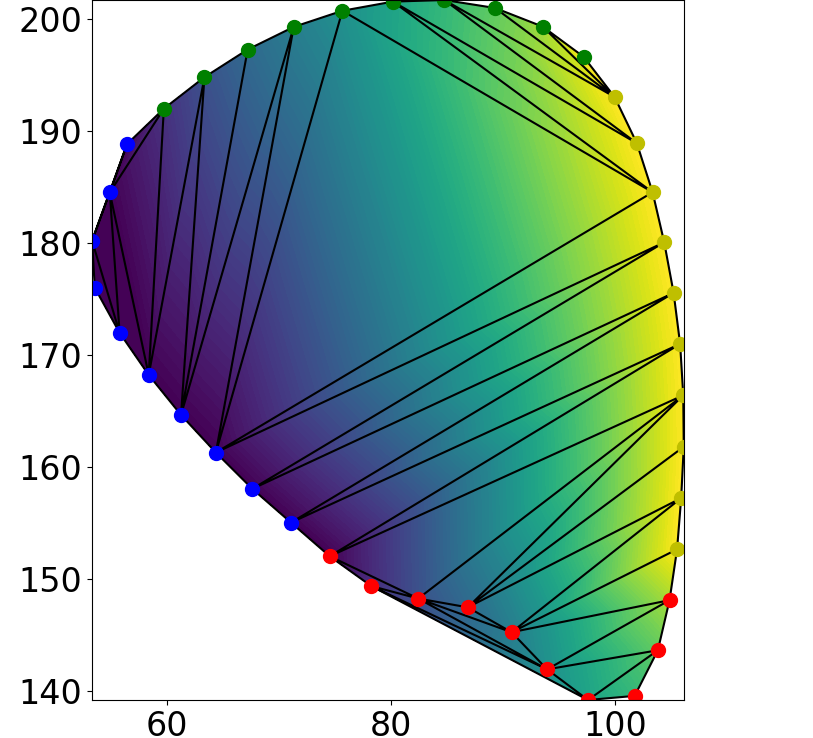
\includegraphics[width=\textwidth]{images/fiber_creation/u_0.png}%
    \caption{First method,\\Quickhull agorithm}%
    \label{fig:triu_0}%
  \end{subfigure}
  \quad
  \begin{subfigure}[t]{0.31\textwidth}%
    \centering%
    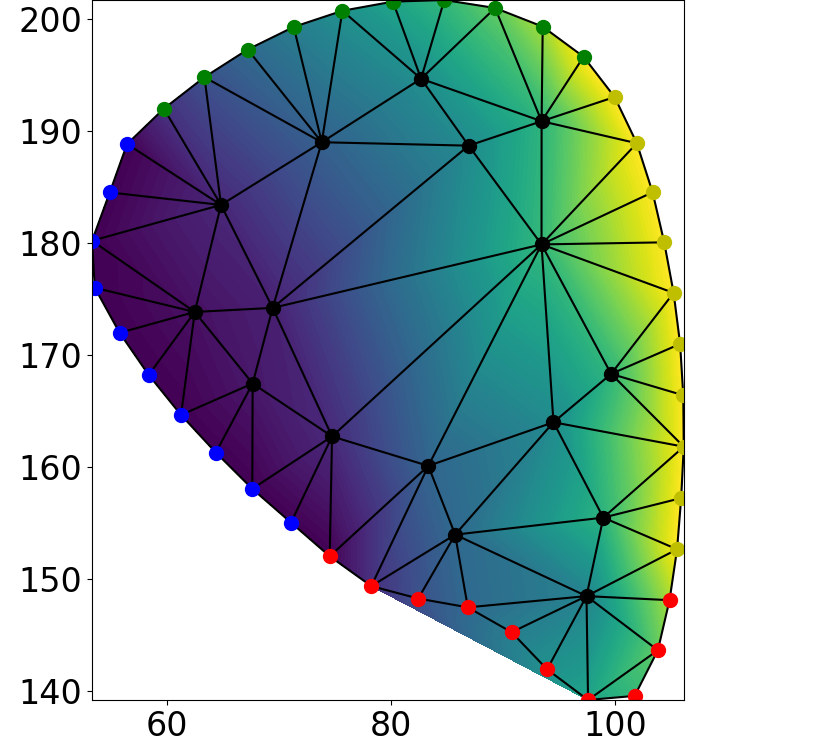
\includegraphics[width=\textwidth]{images/fiber_creation/u_1.png}%
    \caption{Second method,\\Delaunay refinement}%
    \label{fig:triu_1}%
  \end{subfigure}
  \quad
  \begin{subfigure}[t]{0.31\textwidth}%
    \centering%
    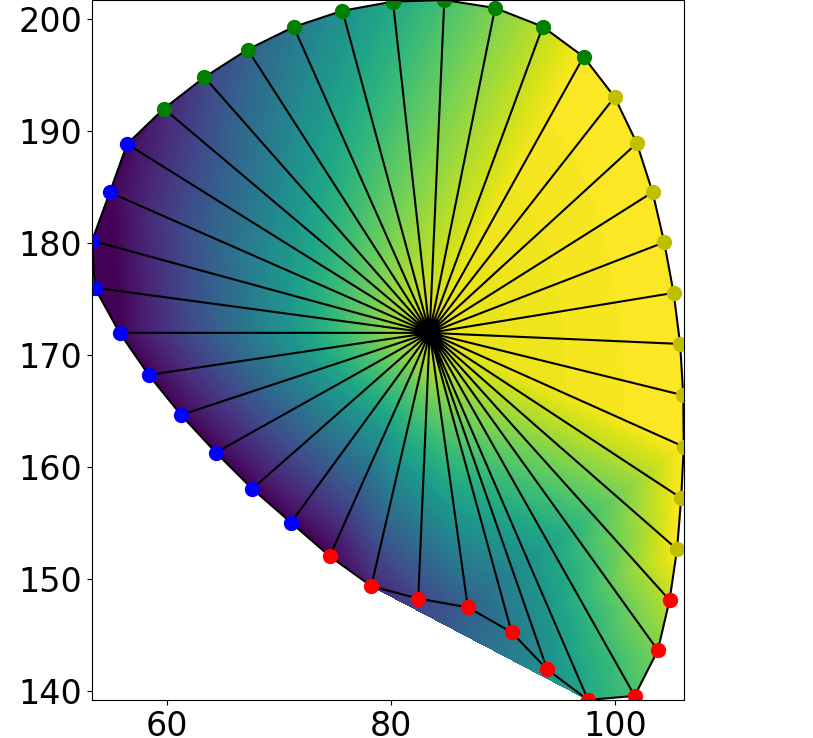
\includegraphics[width=\textwidth]{images/fiber_creation/u_2.png}%
    \caption{Third method,\\center of gravity}%
    \label{fig:triu_2}%
  \end{subfigure}\\
  
  % square
  \begin{subfigure}[t]{0.31\textwidth}%
    \centering%
    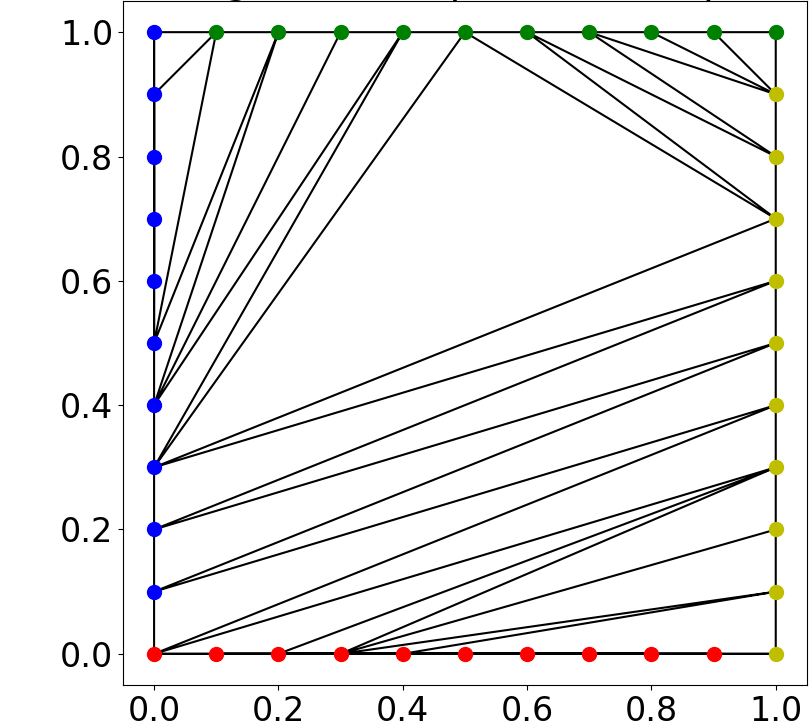
\includegraphics[width=0.9\textwidth, trim=37mm 14mm 6mm 6mm, clip]{images/fiber_creation/mesh_plots/out_0_1_0_tri.png}%
    %\caption{}%
    \label{fig:w_01}%
  \end{subfigure}
  \quad
  \begin{subfigure}[t]{0.31\textwidth}%
    \centering%
    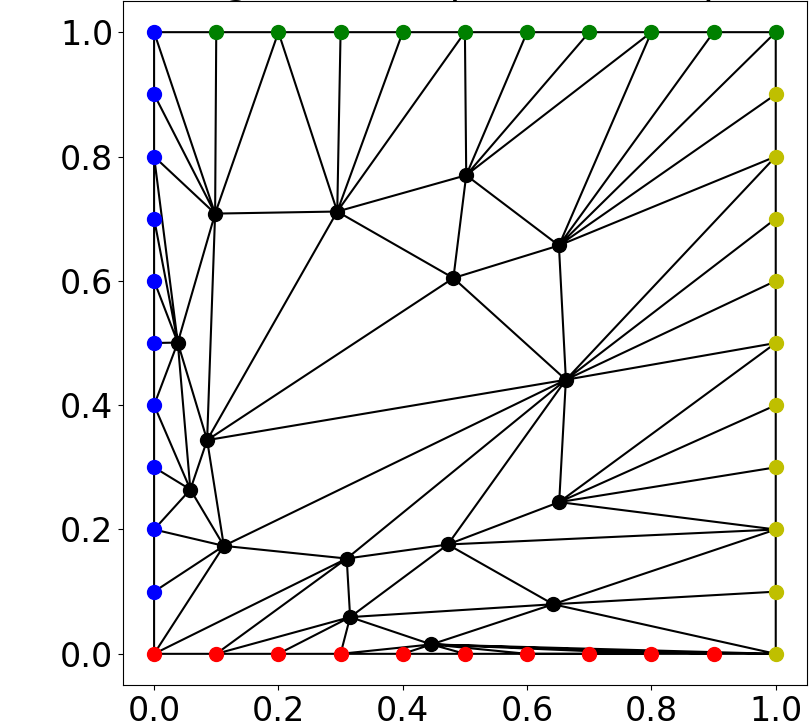
\includegraphics[width=0.9\textwidth, trim=37mm 14mm 6mm 6mm, clip]{images/fiber_creation/mesh_plots/out_1_1_0_tri.png}%
    %\caption{}%
    \label{fig:w_11}%
  \end{subfigure}
  \quad
  \begin{subfigure}[t]{0.31\textwidth}%
    \centering%
    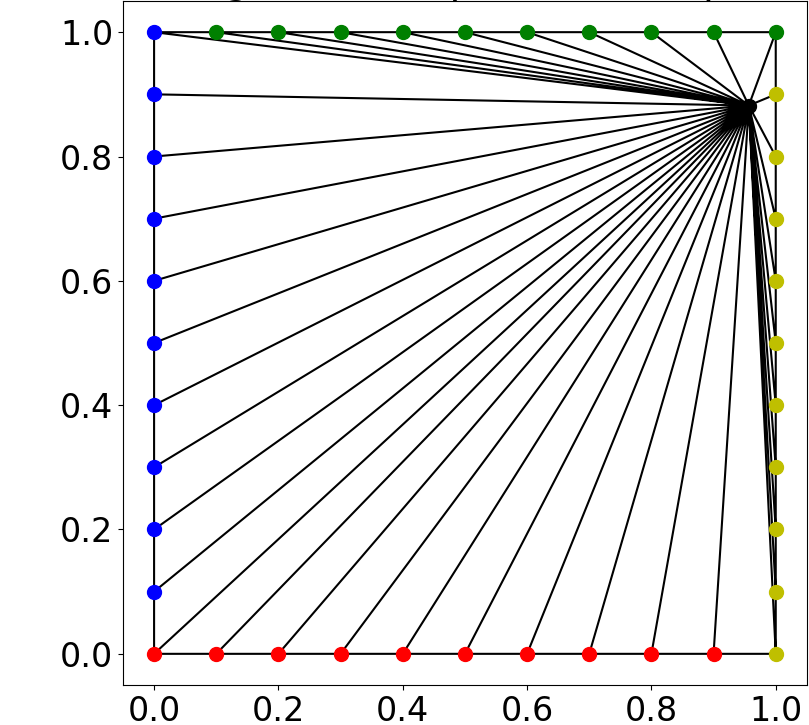
\includegraphics[width=0.9\textwidth, trim=37mm 14mm 6mm 6mm, clip]{images/fiber_creation/mesh_plots/out_2_1_0_tri.png}%
    %\caption{}%
    \label{fig:w_21}%
  \end{subfigure}\\
  
  % circle
  \hspace{-12mm}
  \begin{subfigure}[t]{0.31\textwidth}%
    \centering%
    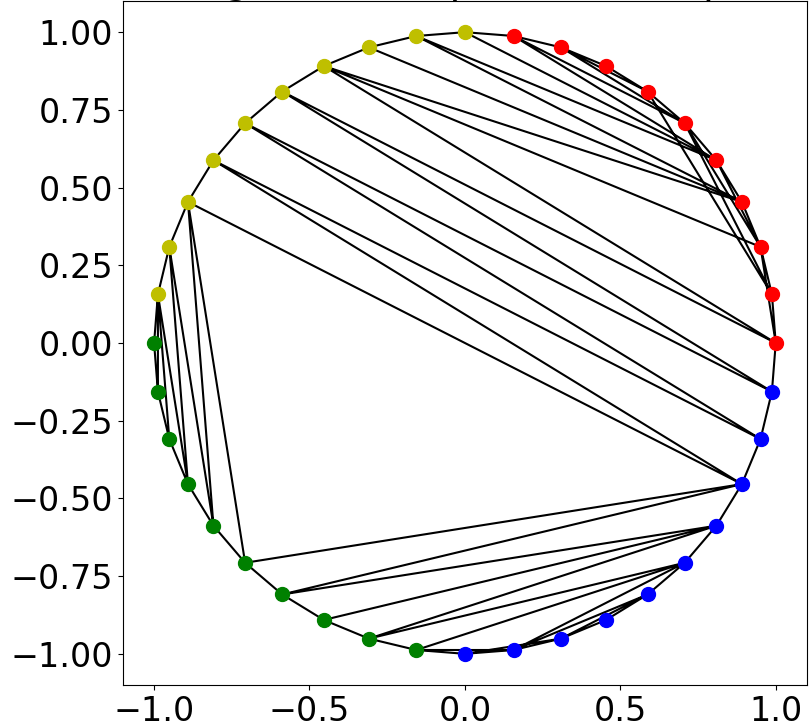
\includegraphics[width=0.9\textwidth, trim=37mm 14mm 6mm 6mm, clip, angle=225,origin=c]{images/fiber_creation/mesh_plots/out_0_0_0_tri.png}% trim=left bottom right top, clip]
    %\caption{}%
    \label{fig:w_00}%
  \end{subfigure}
  \quad
  \begin{subfigure}[t]{0.31\textwidth}%
    \centering%
    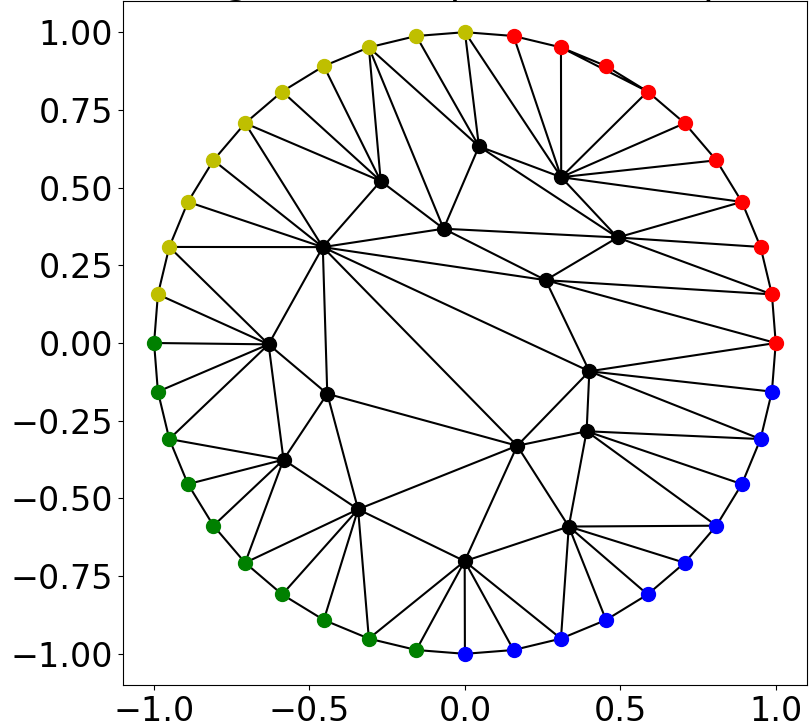
\includegraphics[width=0.9\textwidth, trim=37mm 14mm 6mm 6mm, clip, angle=225,origin=c]{images/fiber_creation/mesh_plots/out_1_0_0_tri.png}%
    %\caption{}%
    \label{fig:w_10}%
  \end{subfigure}
  \quad
  \begin{subfigure}[t]{0.31\textwidth}%
    \centering%
    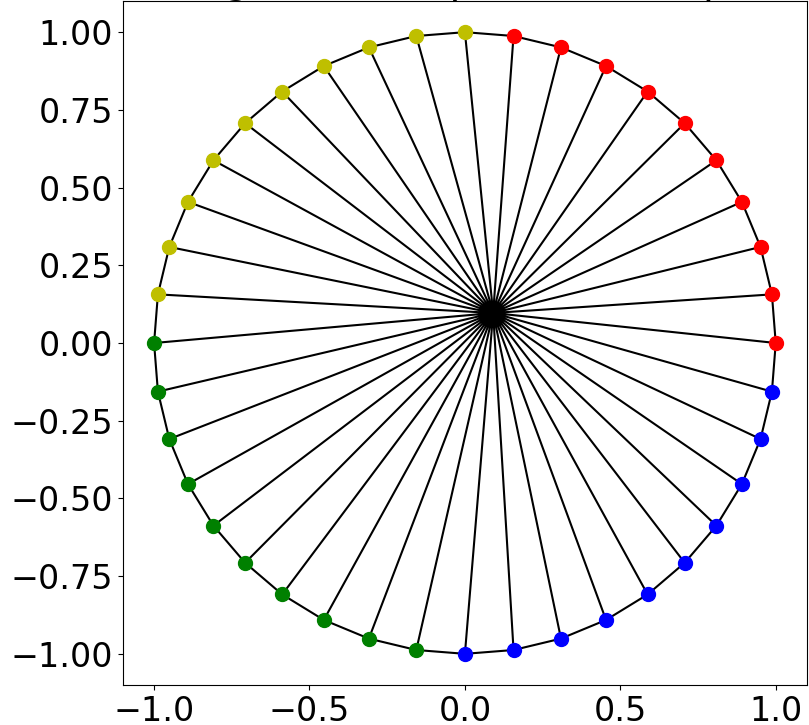
\includegraphics[width=0.9\textwidth, trim=37mm 14mm 6mm 6mm, clip, angle=225,origin=c]{images/fiber_creation/mesh_plots/out_2_0_0_tri.png}%
    %\caption{}%
    \label{fig:w_20}%
  \end{subfigure}
  
  \caption{Top row: Different triangulation methods for $S_M$, the color represents the solution $u$ of the harmonic map. Middle and bottom row: triangulation mapped to the parameter domain $\Omega_P$, for the unit square (middle) and the unit circle (bottom). Each column corresponds to one triangulation method.}%
  \label{fig:tri_triangulations}%
\end{figure}%



In the next step, the algorithm creates a quadrilateral mesh in the parameter domain and computed its image in the muscle domain using the inverse of the harmonic map. The results are shown in \cref{fig:tri_meshes} for the different triangulation methods (columns) and for four different schemes to create the quadrilateral mesh (rows).

In the images in column (\subref{fig:tu_2}) and rows (\subref{fig:tquad_1}) and (\subref{fig:tquad_2}) it can be seen that the previously observed effect with a bad mapping for squares and the third triangulation methods also leads to a mesh in $S_M$ of poor quality.

The two square schemes in rows (\subref{fig:tquad_1}) and (\subref{fig:tquad_2}) show similar results. In the example, good results using the square reference domain are only observed for the first triangulation method.

It can be seen that the approximation quality of the border of the domain varies for some schemes. Especially the combination of the first triangulation method and the square parameter domain, which is known to produce degenerate triangles, poorly reproduces the shape of the slice. The mismatch occurs mainly at the red border points, where the original slice has its concavity. Furthermore, also the parameter mesh in the unit circle generated by scheme 1 produces an inaccurate representation of the border. In this case, the reason is not a bad mapping but the low number of elements at the border.

The two schemes for the circle parameter domain in rows (\subref{fig:tquad_3}) and (\subref{fig:tquad_4}) both generate reasonable meshes for all triangulation methods, despite the different structured of the generated meshes. The best results for both schemes occur with the third triangulation method.

% ------------------
% resulting meshes
\begin{figure}%
  \centering%
  \hspace{0.24\textwidth}
  \begin{subfigure}[t]{0.24\textwidth}%
    \centering%
    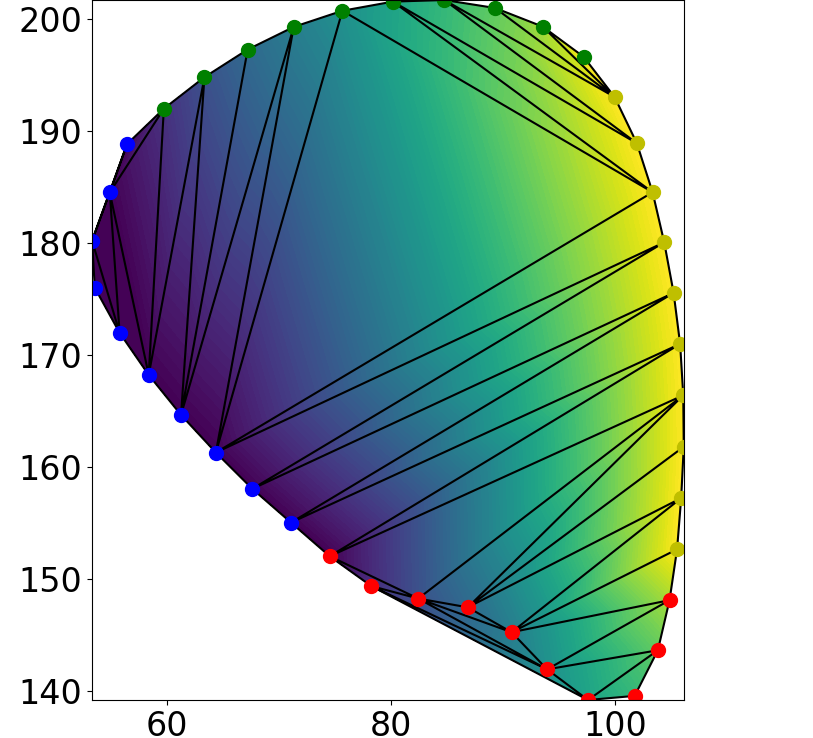
\includegraphics[width=\textwidth]{images/fiber_creation/u_0.png}%
    \caption{First method}%
    \label{fig:tu_0}%
  \end{subfigure}
  \begin{subfigure}[t]{0.24\textwidth}%
    \centering%
    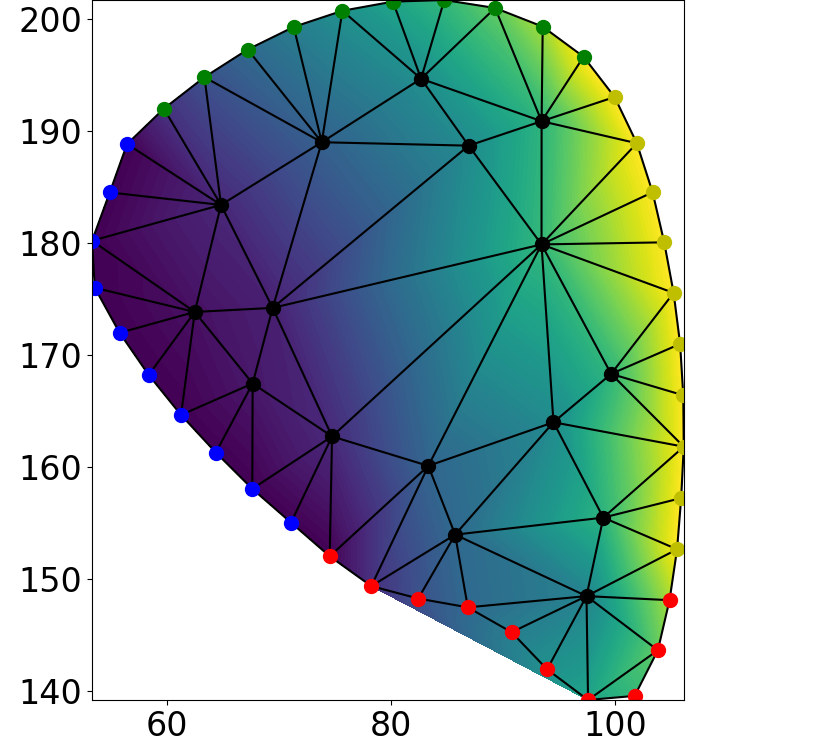
\includegraphics[width=\textwidth]{images/fiber_creation/u_1.png}%
    \caption{Second method}%
    \label{fig:tu_1}%
  \end{subfigure}
  \begin{subfigure}[t]{0.24\textwidth}%
    \centering%
    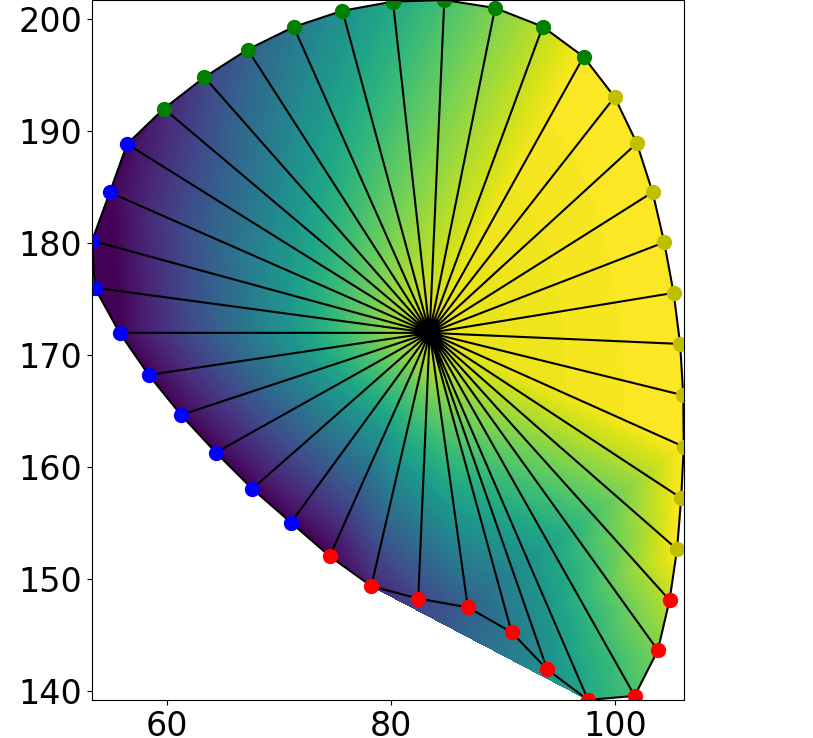
\includegraphics[width=\textwidth]{images/fiber_creation/u_2.png}%
    \caption{Third method}%
    \label{fig:tu_2}%
  \end{subfigure}\\
  
  % square
  \begin{subfigure}[t]{0.24\textwidth}%
    \centering%
    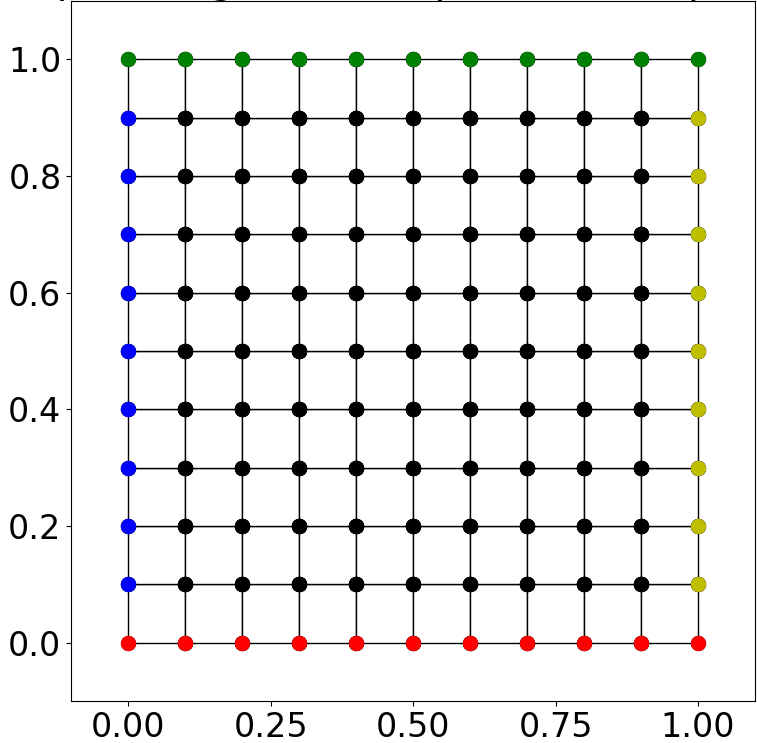
\includegraphics[width=\textwidth]{images/fiber_creation/quad_1.png}%
    \caption{Square, scheme 1}%
    \label{fig:tquad_1}%
  \end{subfigure}
  \begin{subfigure}[t]{0.24\textwidth}%
    \centering%
    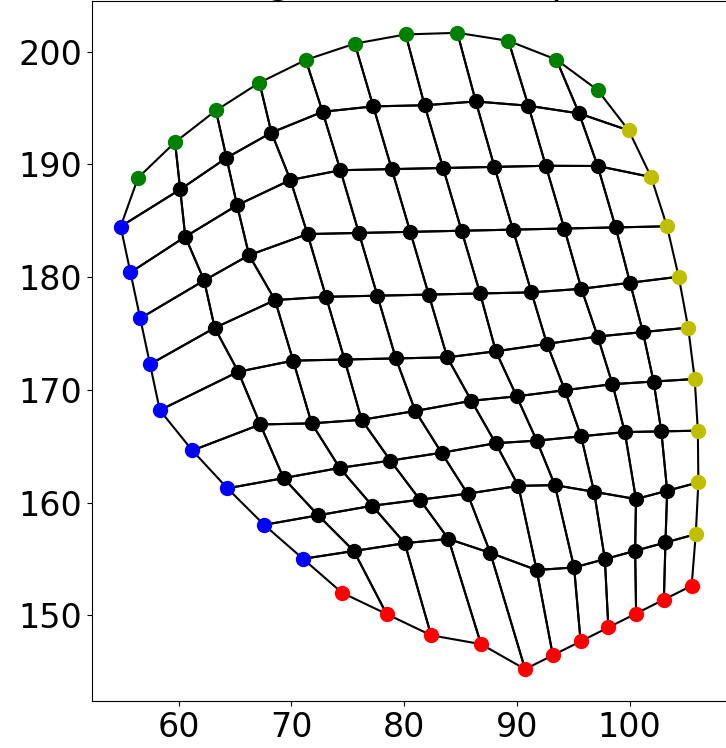
\includegraphics[width=\textwidth, trim=26mm 14mm 6mm 6mm, clip]{images/fiber_creation/mesh_plots/out_0_1_0_w.png}%
    %\caption{}%
    \label{fig:tri_01}%
  \end{subfigure}
  \begin{subfigure}[t]{0.24\textwidth}%
    \centering%
    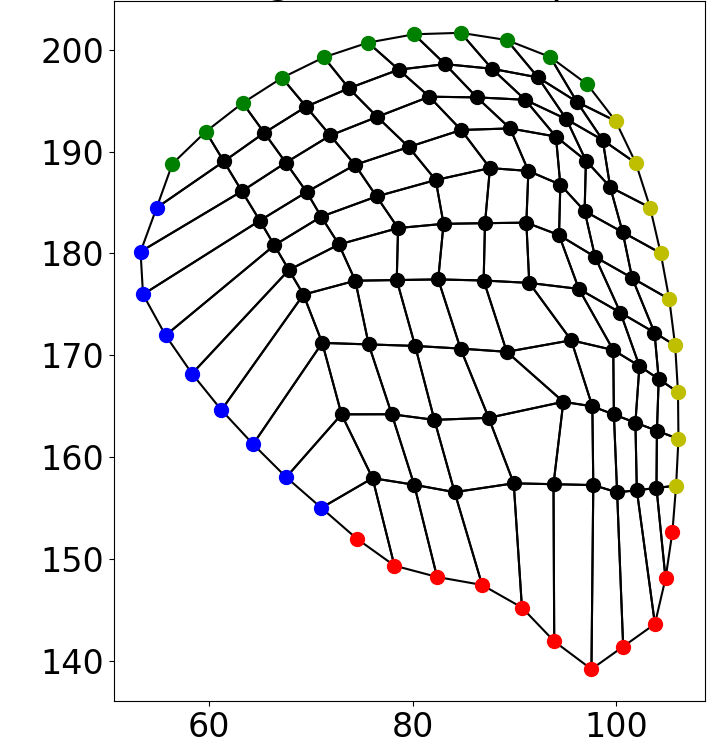
\includegraphics[width=\textwidth, trim=30mm 14mm 6mm 6mm, clip]{images/fiber_creation/mesh_plots/out_1_1_0_w.png}%
    %\caption{}%
    \label{fig:tri_11}%
  \end{subfigure}
  \begin{subfigure}[t]{0.24\textwidth}%
    \centering%
    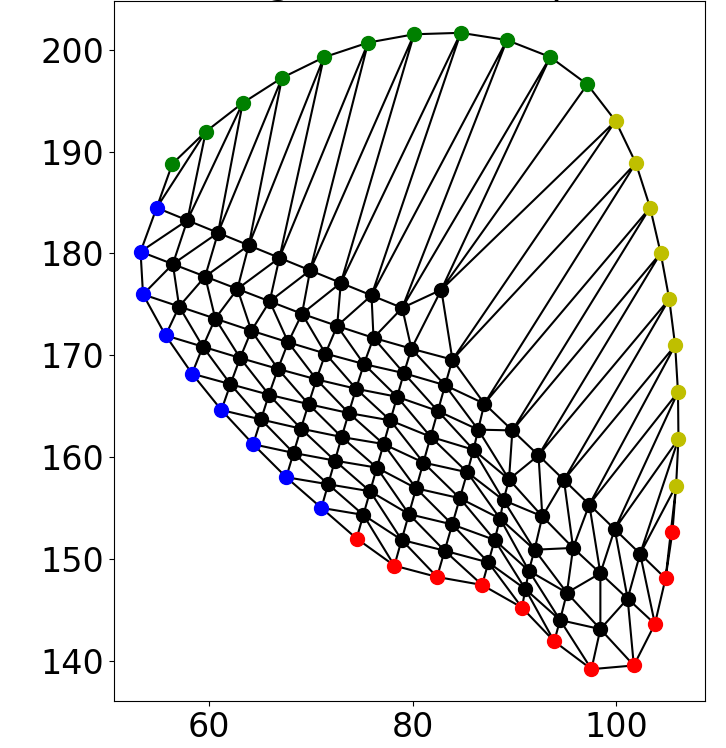
\includegraphics[width=\textwidth, trim=30mm 14mm 6mm 6mm, clip]{images/fiber_creation/mesh_plots/out_2_1_0_w.png}%
    %\caption{}%
    \label{fig:tri_21}%
  \end{subfigure}\\[-4mm]
  
  % square adjusted
  \begin{subfigure}[t]{0.24\textwidth}%
    \centering%
    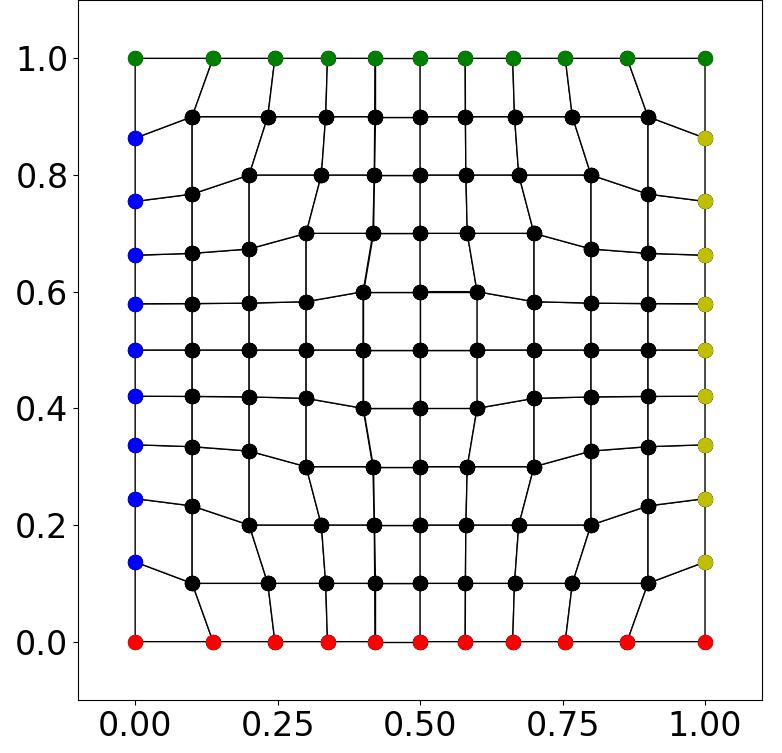
\includegraphics[width=\textwidth]{images/fiber_creation/quad_2.png}%
    \caption{Square, scheme 2}%
    \label{fig:tquad_2}%
  \end{subfigure}
  \begin{subfigure}[t]{0.24\textwidth}%
    \centering%
    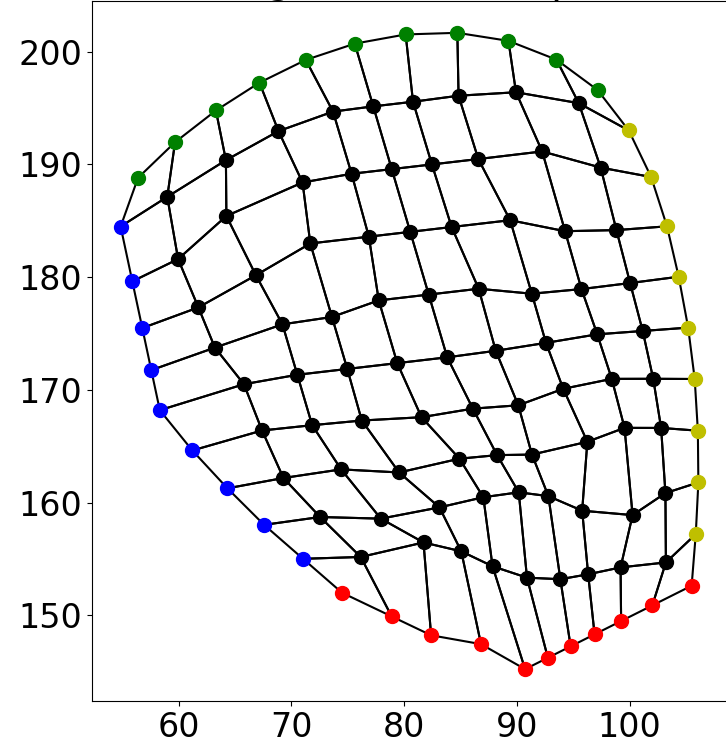
\includegraphics[width=\textwidth, trim=26mm 14mm 6mm 6mm, clip]{images/fiber_creation/mesh_plots/out_0_2_0_w.png}%
    %\caption{}%
    \label{fig:tri_02}%
  \end{subfigure}
  \begin{subfigure}[t]{0.24\textwidth}%
    \centering%
    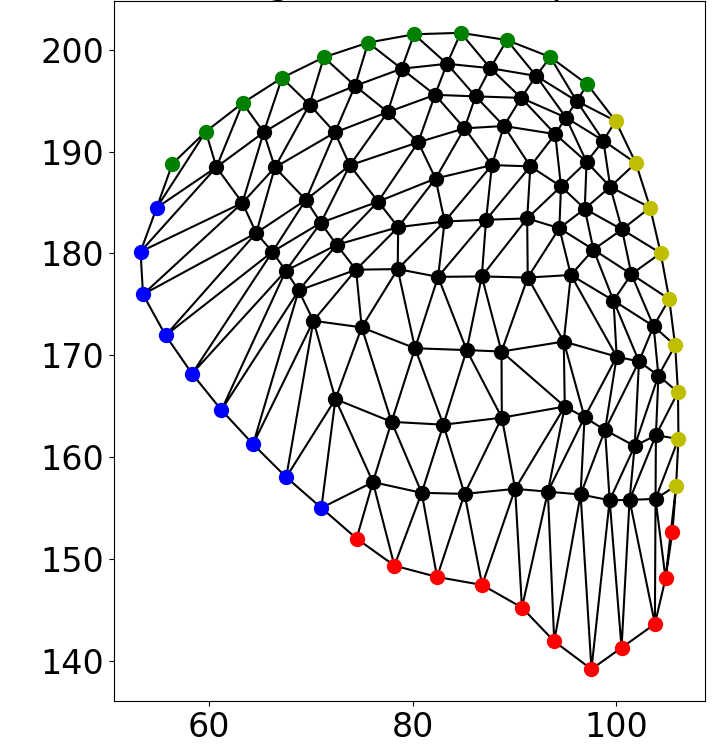
\includegraphics[width=\textwidth, trim=30mm 14mm 6mm 6mm, clip]{images/fiber_creation/mesh_plots/out_1_2_0_w.png}%
    %\caption{}%
    \label{fig:tri_12}%
  \end{subfigure}
  \begin{subfigure}[t]{0.24\textwidth}%
    \centering%
    \includegraphics[width=\textwidth, trim=30mm 14mm 6mm 6mm, clip]{images/fiber_creation/mesh_plots/out_2_2_0_w.png}%
    %\caption{}%
    \label{fig:tri_22}%
  \end{subfigure}\\[-4mm]
  
  % circle
  \begin{subfigure}[t]{0.24\textwidth}%
    \centering%
    \includegraphics[width=\textwidth]{images/fiber_creation/quad_0.png}%
    \caption{Circle, scheme 1}%
    \label{fig:tquad_0}%
  \end{subfigure}
  \begin{subfigure}[t]{0.24\textwidth}%
    \centering%
    \includegraphics[width=\textwidth, trim=26mm 14mm 6mm 6mm, clip]{images/fiber_creation/mesh_plots/out_0_0_0_w.png}% trim=left bottom right top, clip]
    %\caption{}%
    \label{fig:tri_00}%
  \end{subfigure}
  \begin{subfigure}[t]{0.24\textwidth}%
    \centering%
    \includegraphics[width=\textwidth, trim=26mm 14mm 6mm 6mm, clip]{images/fiber_creation/mesh_plots/out_1_0_0_w.png}%
    %\caption{}%
    \label{fig:tri_10}%
  \end{subfigure}
  \begin{subfigure}[t]{0.24\textwidth}%
    \centering%
    \includegraphics[width=\textwidth, trim=30mm 14mm 6mm 6mm, clip]{images/fiber_creation/mesh_plots/out_2_0_0_w.png}%
    %\caption{}%
    \label{fig:tri_20}%
  \end{subfigure}\\[-4mm]
  
  % circle adjusted
  \begin{subfigure}[t]{0.24\textwidth}%
    \centering%
    \includegraphics[width=\textwidth]{images/fiber_creation/quad_3.png}%
    \caption{Circle, scheme 2}%
    \label{fig:lquad_3}%
  \end{subfigure}
  \begin{subfigure}[t]{0.24\textwidth}%
    \centering%
    \includegraphics[width=\textwidth, trim=30mm 14mm 6mm 6mm, clip]{images/fiber_creation/mesh_plots/out_0_3_0_w.png}%
    %\caption{}%
    \label{fig:tri_03}%
  \end{subfigure}
  \begin{subfigure}[t]{0.24\textwidth}%
    \centering%
    \includegraphics[width=\textwidth, trim=30mm 14mm 6mm 6mm, clip]{images/fiber_creation/mesh_plots/out_1_3_0_w.png}%
    %\caption{}%
    \label{fig:tri_13}%
  \end{subfigure}
  \begin{subfigure}[t]{0.24\textwidth}%
    \centering%
    \includegraphics[width=\textwidth, trim=30mm 14mm 6mm 6mm, clip]{images/fiber_creation/mesh_plots/out_2_3_0_w.png}%
    %\caption{}%
    \label{fig:tri_23}%
  \end{subfigure}
  \caption{Meshes in $S_M$ for quadrangulations (rows) and triangulations (columns).}%
  \label{fig:tri_meshes}%
\end{figure}%

% quantitative quality plots of results
For a quantitative comparison of the results, the different variants were executed for 43 slices of the biceps muscle, resulting in 43 meshes for every combination of triangulation method and quadrangulation scheme.

In each generated mesh the edge lengths of the elements were collected and normalized to have a mean of 1. The normalization is required to allow a comparison between meshes with different bounding boxes.
The standard deviation of the normalized lengths was determined in each mesh. The total mean of all the standard deviations was computed. This value is a measured for the quality of the mesh. A low value means that in every slice the generated mesh has similar edge length and, in consequence, the overall meshing has good quality.

\begin{figure}%
  \centering%
  \includegraphics[width=\textwidth]{images/fiber_creation/mesh_quality.pdf}%
  \caption{Mesh quality (red, lower is better) and duration (yellow) for the three different triangulation methods and the different parameter space quadrangulation schemes. A low value for the standard deviation of relative element lengths indicates good quality.}%
  \label{fig:mesh_quality}%
\end{figure}

\Cref{fig:mesh_quality} visualizes the results. Three groups of bars are displayed for the three triangulation methods. For every type of mesh in the parameter space, i.e. unit square ($\square$) or unit circle ($\ocircle$) and scheme 1 or 2, the standard deviation is given by the red bar and the duration of the overall algorithm is given by the yellow bar. The corresponding axis labels for standard deviation and duration are given on the left and right of the diagram.

The diagram shows the lowest standard deviation of edges and therefore the best mesh quality for the first triangulation method and the square, with scheme 1 having a slightly better value than scheme 2. This shows that the modified placement of the nodes in scheme 2 has no positive effect compared to scheme 1.
However, from the observations in \cref{tri_triangulations} it is known that the borders may be approximated poorly. This does not influence the chosen metric of uniform relative edge lengths.
Similar good results can be seen for scheme 2 in the circular parameter domain and the second and third triangulations.

Moreover, it can be seen that certain connections between parameter domain and suited triangulation scheme exist. The square parameter domain works best with the first triangulation method. The second scheme for the parameter mesh on the unit circle works best with the triangulation methods 2 and 3.

The first scheme for the parameter mesh on the unit circle shows a bad results for all triangulation methods. This can be explained by looking at the generated meshes in row (\subref{fig:tquad_0}) of \cref{fig:tri_meshes}. By construction, the elements have a bad aspect ratio. This results in the high standard deviation values. However, the generated meshes still look uniform to a certain extent and can be useful in applications where such type of mesh is needed. The score could be improved by adding more nodes in circumferential direction.

The runtime of the algorithm is approximately the same for the different parameter domain meshes. It mainly depends on the triangulation of the slices. The first triangulation using the \emph{scipy} package takes the most time, followed by the Delaunay refinement. The fastest triangulation is the custom one where only one additional point needs to be placed. In conclusion, when runtime is an issue, the third triangulation should be chosen. It achieves good quality meshes only with the second scheme of the circular parameter domain. This combination also does not suffer from the bad approximation quality of the border, as is the case for the unit circle with the first triangulation method.

\section{Parallel Algorithm to Create Muscle and Fiber Meshes}\label{sec:parallel_algorithm}
parallel algorihm

% (Laplacian smoothing)
%\cite{field1988laplacianSmoothingAndDelaunayTriangulations}

\begin{algorithm}
  \begin{algorithmic}[1]%
    \Procedure{Create\_3D\_meshes\_parallel}{}
    \Require triangulated tubular surface
    \Ensure structured 3D volume mesh
    \Ensure 1D fiber meshes
    \Statex
    \State Solve Laplacian flow problem
    \State Trace streamlines in the gradient field
    \State Sample 1D fiber meshes
    \EndProcedure
  \end{algorithmic}%
  \caption{Parallel algorithm}%
  \label{alg:parallel_algorithm_1}%
\end{algorithm}%


\section{Results and Discussion}

conclusion for automatic segmentation: doesn't work for muscles, only for bones

If the quality of the images should be improved, it is also possible to manually edit the intermediate results of segmentations.
